\documentclass[journal]{IEEEtran}

\usepackage{newtxtext,newtxmath}
\usepackage{mathrsfs}
\usepackage{graphicx}

% Packages for figures and subfigures:
\usepackage{caption}
\usepackage{subcaption}
\usepackage{multicol}

% Commenting out large sections for drafts
\usepackage{verbatim}

\begin{document}

\title{Investigating the alignment of stellar halos with cosmic web filaments using the nIFTy cluster}

\author{Emily Hackett,~\IEEEmembership{Bachelor of Philosophy (Honours) Student, UWA}}% <-this % stops a space
	
% The paper headers
\markboth{Proceedings of the Pawsey Supercomputing Centre Summer Internships,~Vol.~1, No.~1, February~2017}%
{Shell \MakeLowercase{\textit{et al.}}: Alignment of stellar halos with filaments}
% The only time the second header will appear is for the odd numbered pages
% after the title page when using the twoside option.

% make the title area
\maketitle

%%%%% ABSTRACT %%%%%
\begin{abstract}
	Previous research has shown that the structural properties of dark matter haloes can correlate with their local environment (such as filaments and voids), as similarly those of baryonic galaxies may also do, although to a lesser extent. The significance of characterising these sorts of correlation is their relationship to the theory of hierarchical structure formation in large-scale structure (as well as possibly substructure), as it can be used todemonstrate the influence of major mergers on the structural properties of halos. The question this project aims to address is whether a similar correlation between large-scale cosmic web structure and physical characteristics of the smaller embedded structure exists for stellar halos. The stellar halo of a galaxy is an area in which this trend may be more easily examined in coming years with the use of new radio astronomy techniques as well as weak gravitational lensing. Shape properties for these stellar halos can be derived similarly to those for dark matter halos, by calculating the reduced moment of inertia tensor whose eigenvalues and eigenvectors correspond to elliptic major,intermediate and minor axes (from which values for sphericity, triaxiality and ellipticity can be deduced). These values can then be compared to the filamentary structure around and through the halo, which is defined as its' local environment, and measured using the DisPerSe program. This paper aims to analyis the nIFTy cluster, a simulated dark matter halo in a snapshot of the cosmic web, and to examine the possibility of using these techniques on large simulation volumes with multiple halos, such as the Horizon-AGN simulation. 
	(---results---)
\end{abstract}

\begin{IEEEkeywords}
large-scale structure, stellar halo, galaxy formation, hierarchical structure formation
\end{IEEEkeywords}

\IEEEpeerreviewmaketitle

%%%%% INTRO %%%%%
\section{Introduction}
\IEEEPARstart{T}{hrough} analysis of N-body hydrodynamical simulations in cold dark matter (CDM) cosmologies, clear correlations have been observed between the properties of dark matter haloes and their local environment within the cosmic web. This environment is defined by large-scale structures such as clusters, voids, filaments and sheets, along which the dark matter halo may tend to be aligned parallel or perpendicular. This alignment can be measured with respect to physical properties such as shape (via triaxiality, ellipticity and major/minor axes alignments) or angular momenta and spin. For example, in a hierarchical formation model, it would be expected that halos tend towards prolateness rather than oblateness \cite{bett07} since they are formed by matter collapsing along filaments. 

Another recent trend in cosmological simulations is analysis of the stellar halo, which is seen as . There is a need to develop proper, physical models of galaxy formation within DM halos to use in large-scale cosmological simulations to determine if distributions of galaxies are realistic \cite{davis85}. Large scale structure, such as dark matter filaments, clusters and voids, are a general result of nonlinear evolution models in cold dark matter cosmological simulations. The characteristic scale of clustering in a $\lambda$-CDM universe grows extremely fast, which is computationally difficult, despite the need for greater spatial resolution in simulations in order to investigate galaxy formation. Although simulations allow us to predict mass distributions in the universe, what we are capable of observing is galaxies - therefore it is important to know how galaxies are biased around large-scale structure, a correlation that is possibly influenced by the mechanics of galaxy formation. Modelling and determining the alignments of dark matter in N-body simulations is computationally easier than modelling complex baryonic physics and galaxy formation (even if there existed an agreed upon model). 

%\subsection{Hierarchical Structure Formation}

The fact that these halo properties correlate with the local environment suggests that the baryonic galaxies that form within them likely do so as well \cite{hahn07b}.  Bullock and Johnston \cite{bullock05} propose a way to investigate the properties of galaxies within their local environment by examining the stellar halos of these dark matter halos. These offer an insight into the question of whether structure formation is truly hierarchical on small scales, such as within the stellar halo. If so, abundant substructure would be expected \cite{bullock05}. The reason for using the stellar halo of the dark matter halo - which comprises of all baryonic matter associated with the dark matter halo - as opposed to the smaller, baryonic galaxies scattered within is that the stellar halo will hopefully be less effected by significant merger events along filaments that tend to significantly disrupt samples of galaxies.

%\subsection{Stellar Halos}

\emph{How does the work done on determining origins of stellar halo stars relate to the correlation of the stellar halo with large-scale structure and filaments?}

N-body simulations have been used to determine the relative importance of diffuse accretion verse mergers for halo growth. Observational studies of the metallicity and age of stars in the stellar halo allow similar distinctions to be drawn. In particular, Zolotov et.al. \cite{zolotov09} studied the stellar halo using numerical simulations to determine that it had dual origin: partly from tidal stripping of stars from disrupted satellites, and partly pushed out of the central galaxy in minor mergers. The paper defines the stellar halo as all stellar particles in the region 0.1 $r_{vir}$ to $r_{vir}$ that are not bound to substructures.

At any given redshift, dark matter is clustered on a characteristic mass scale, within which finer substructure is erased by collisions, mergers and tidal effects. \cite{white78} However, luminous material that has condensed in the cores of low-mass halos may in fact survive as the structure collapses and virialises. Hence the stellar halo has the capacity to become a history of sorts of the formation and evolution of its dark matter halo, which is in turn related to the large-scale structure evolving around it. Due to the low surface brightness of halos \cite{zolotov09}, current studies are mostly numerical simulation based rather than observational, although with the advent of the SKA project hopefully new opportunities to compare observations with simulations will become available.

%\subsection{Virial Shocks}

\textit{Add paragraph on what we can expect in terms of structure of a single halo - i.e. what is a viral shock? Why is it important?}

Shock waves develop during the hierarchical evolution of cosmic structures, as the gravitational energy associated with the collapse of dark matter halos (corresponding to galaxy clusters and galaxies) is transformed into the internal energy of the intergalactic medium gaseous components \cite{planelles13}. Mergers and accretion processes then leave signatures on the energetic balance of the shock waves. 


%%% OVERVIEW OF PAPER STRUCTURE %%%%
% Can probably use this in the abstract (along with 2x sentences on background info)

The aim of this project was initially to look at the large-scale hydrodynamical cosmological simulation called the Horizon-AGN \cite{dubois14}, which has been previously used to show that more massive galaxies tend to be oriented perpendicular to the filament, whilst less massive are parallel. This was proposed to be because of the misalignment of galactic angular momentum during mergers, which have occurred with higher frequency in high mass galaxies. However due to time constraints and the lack of a reliable halo-finder algorithm for the huge data set, the analysis was carried out on a single cluster - the nIFTy cluster \cite{nifty}- with the intention of presenting a unified approach to later finding correlations in a large data set. The cluster is plotted for dark matter (DM) and gas densities in Figure \ref{fig:densities} as well as for temperature, using 2D slices in the xy, xz and yz planes respectively. 

In this study, the shape of the dark matter halo (and the corresponding stellar halo) is determined by computing the reduced moment of inertia tensor (see Section II A) for the halo as a whole, assuming an ellipsoidal shape (these eigenvectors and values are related to the direction and length of the principal axes of inertia) \cite{hahn07a}. From this data, shape properties such as sphericity, triaxiality and ellipticity (Section II B) were calculated for the different components as well as the temperature profile. The environment of the cluster is characterised by a filament vector that is calculated from the skeleton produced by the DisPerSe program (see Section II C). The angle between this filament vector and the major axis of the halo is then used to define the alignment of the halo with its large-scale environment, for different components of the halo at increasing radii. 

\begin{figure*}[!t]
\centering
	\begin{subfigure}[t]{0.3\textwidth}
		\centering
		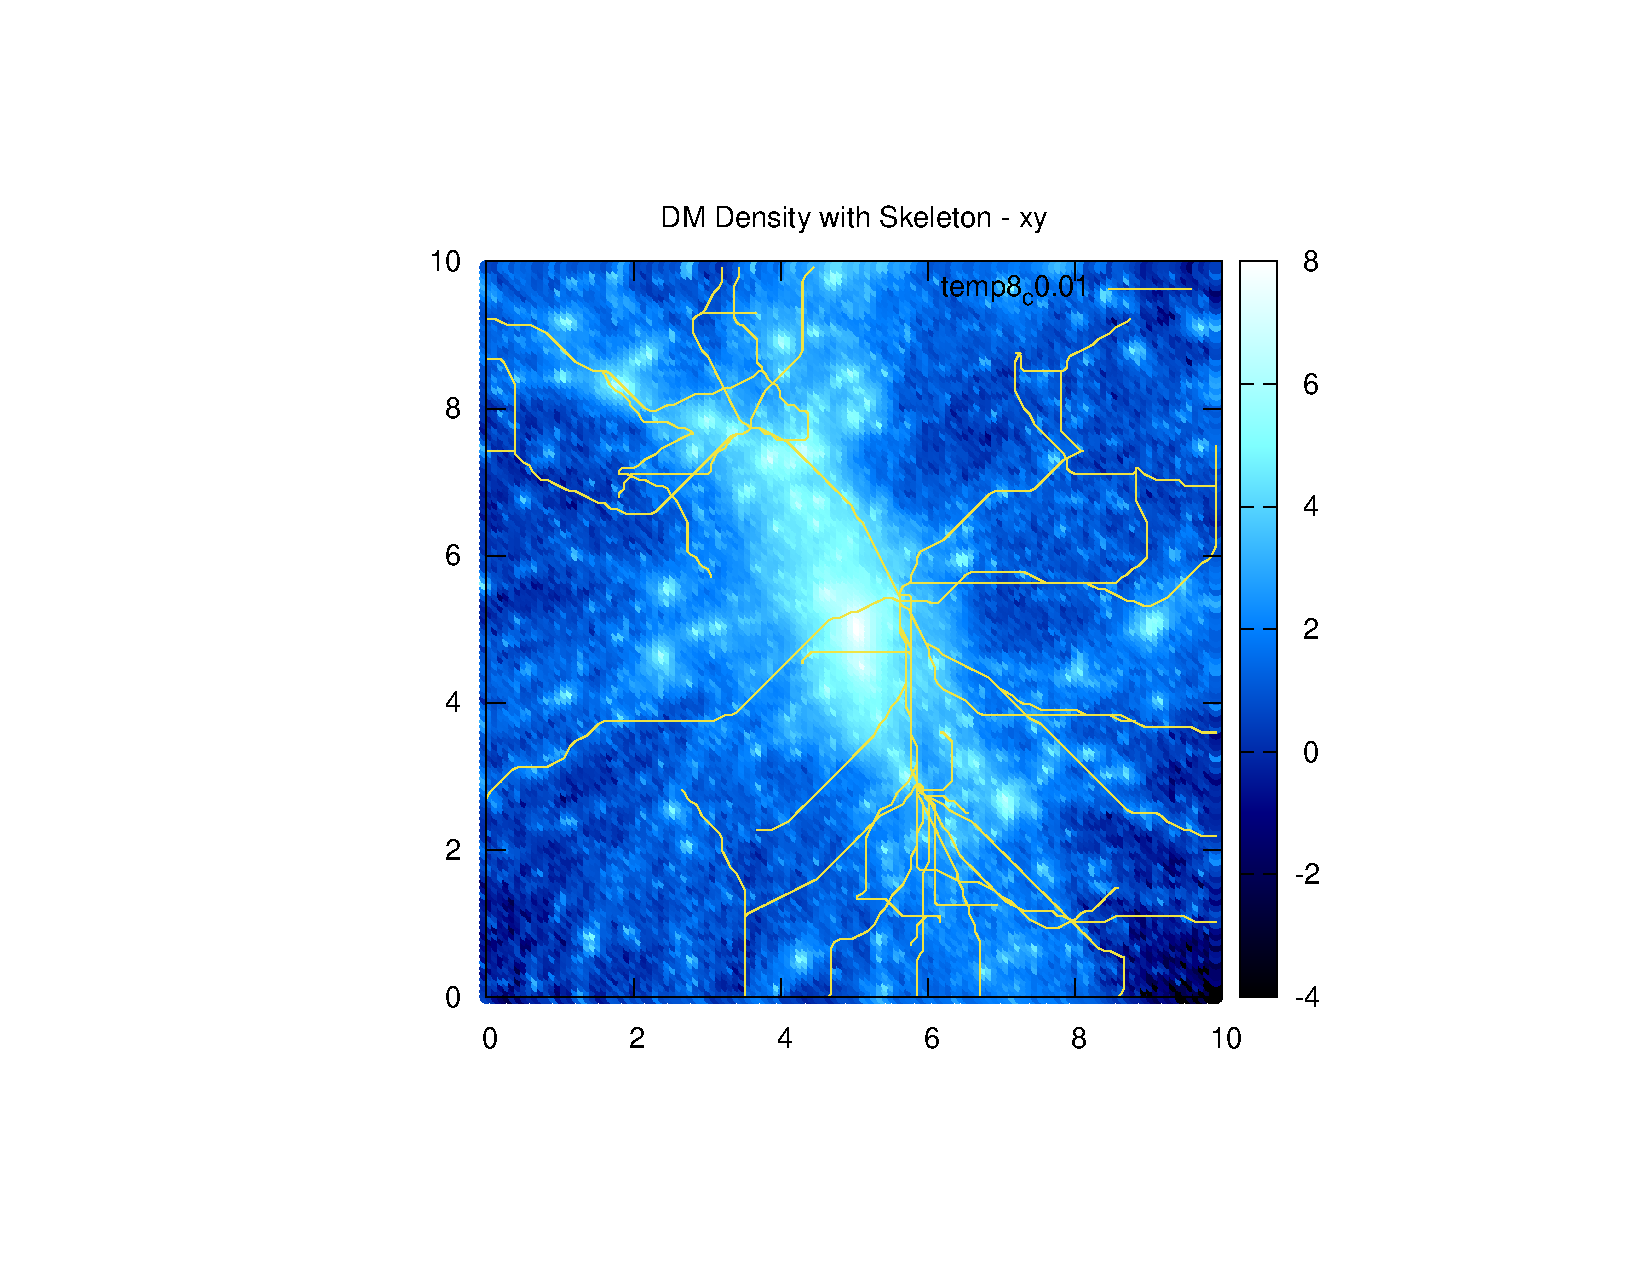
\includegraphics[width=\linewidth]{DMDenSkelxy}
	\end{subfigure}
	\quad
	\begin{subfigure}[t]{0.3\textwidth}
		\centering
		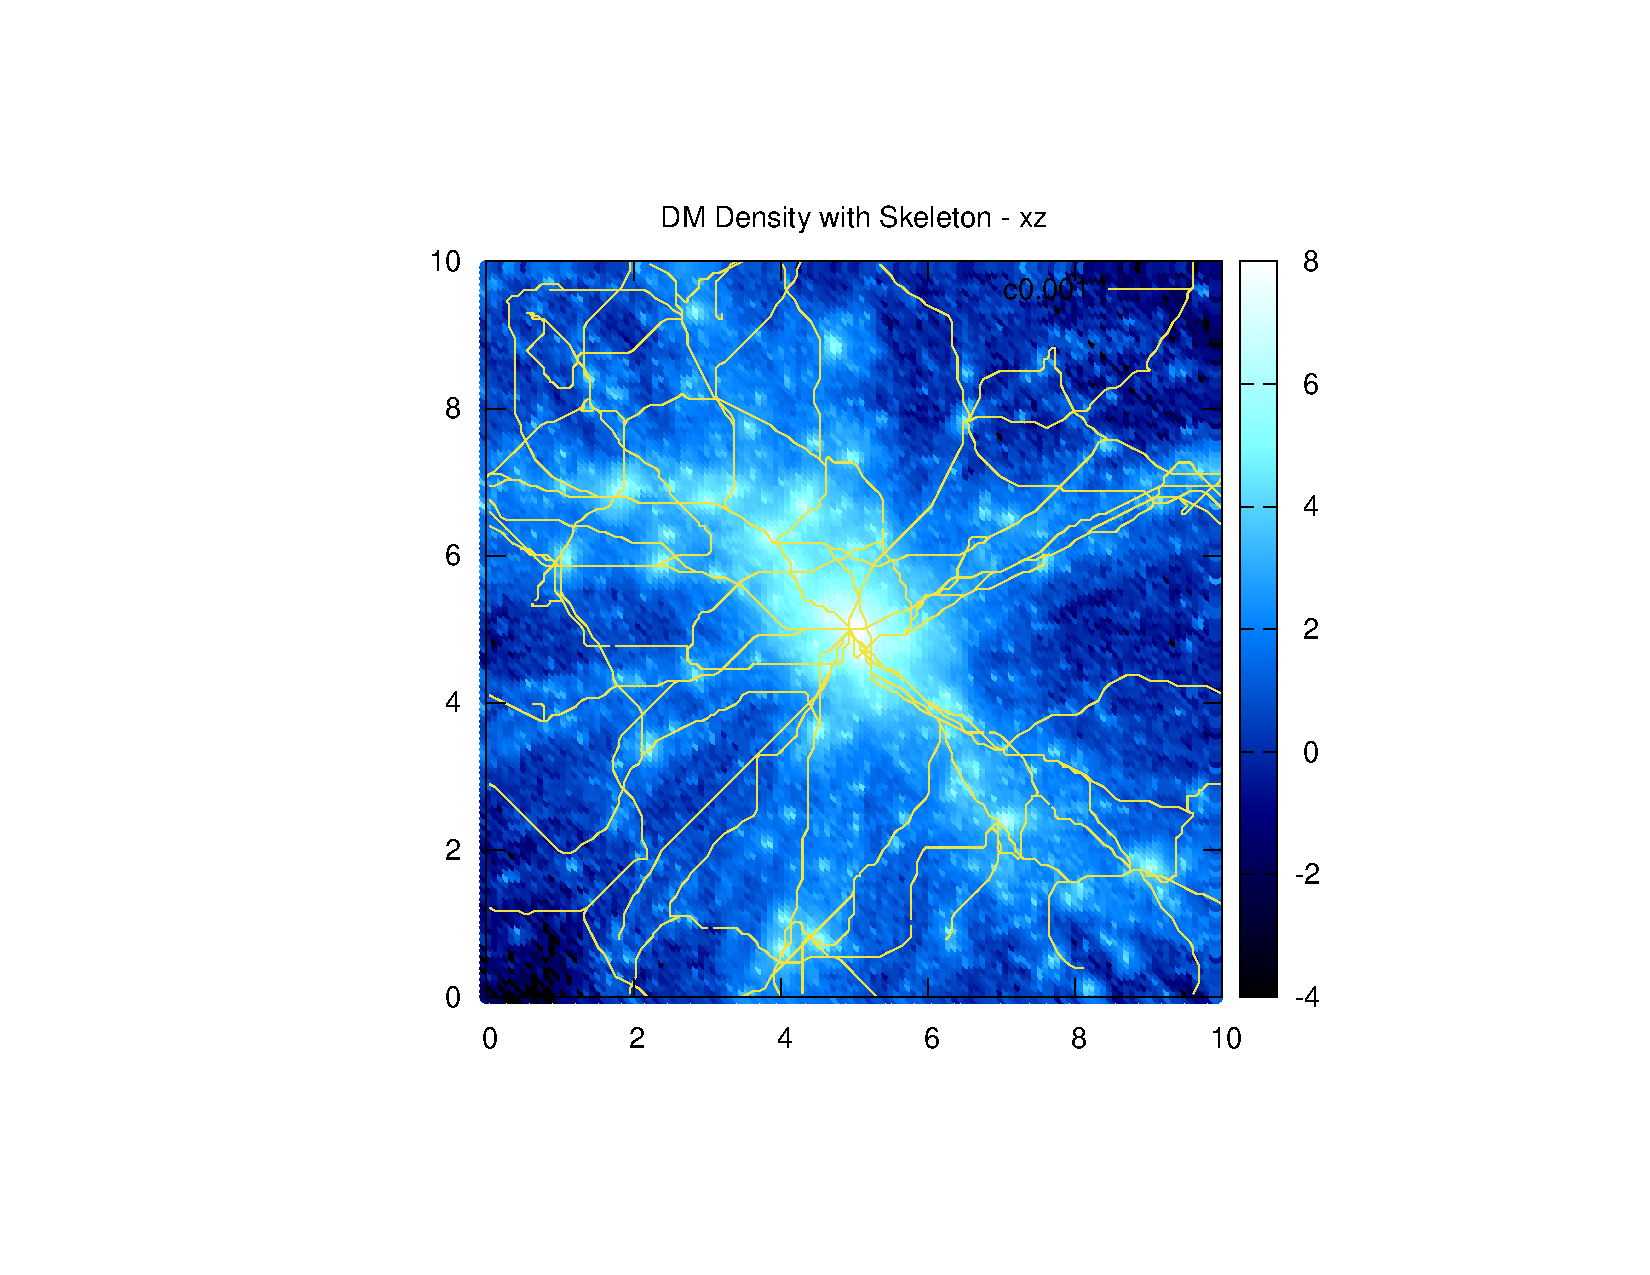
\includegraphics[width=\linewidth]{DMDenSkelxz}
	\end{subfigure}
	\quad
	\begin{subfigure}[t]{0.3\textwidth}
		\centering
		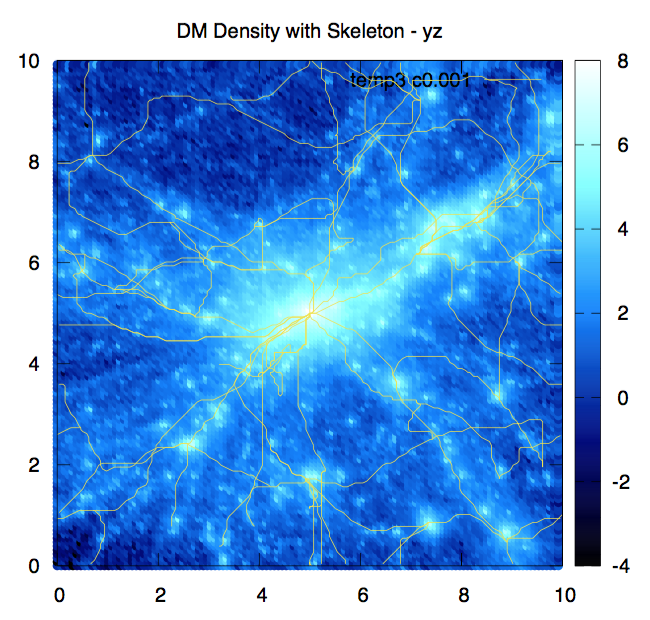
\includegraphics[width=\linewidth]{DMDenSkelyz}
	\end{subfigure}
	\\
	\begin{subfigure}[t]{0.3\textwidth}
		\centering
		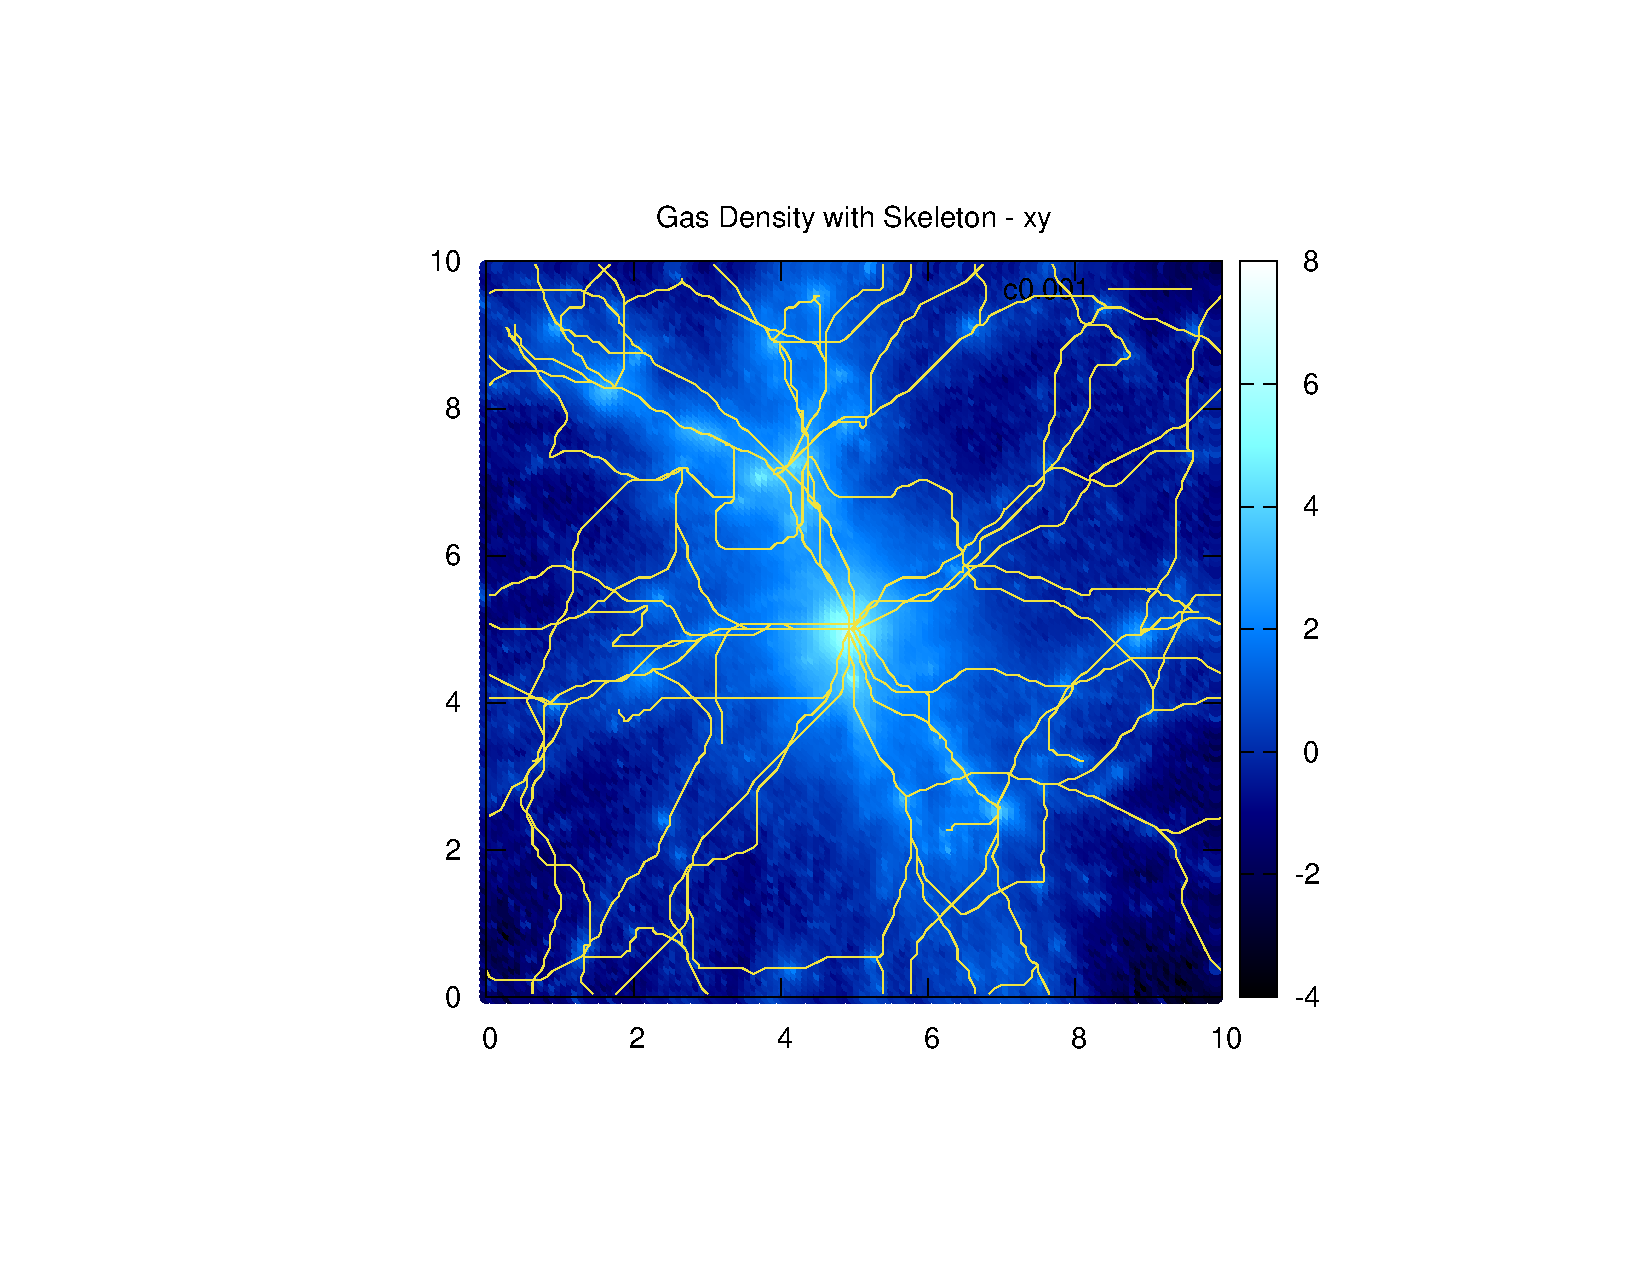
\includegraphics[width=\linewidth]{GasDenSkelxy}
	\end{subfigure}
	\quad
	\begin{subfigure}[t]{0.3\textwidth}
		\centering
		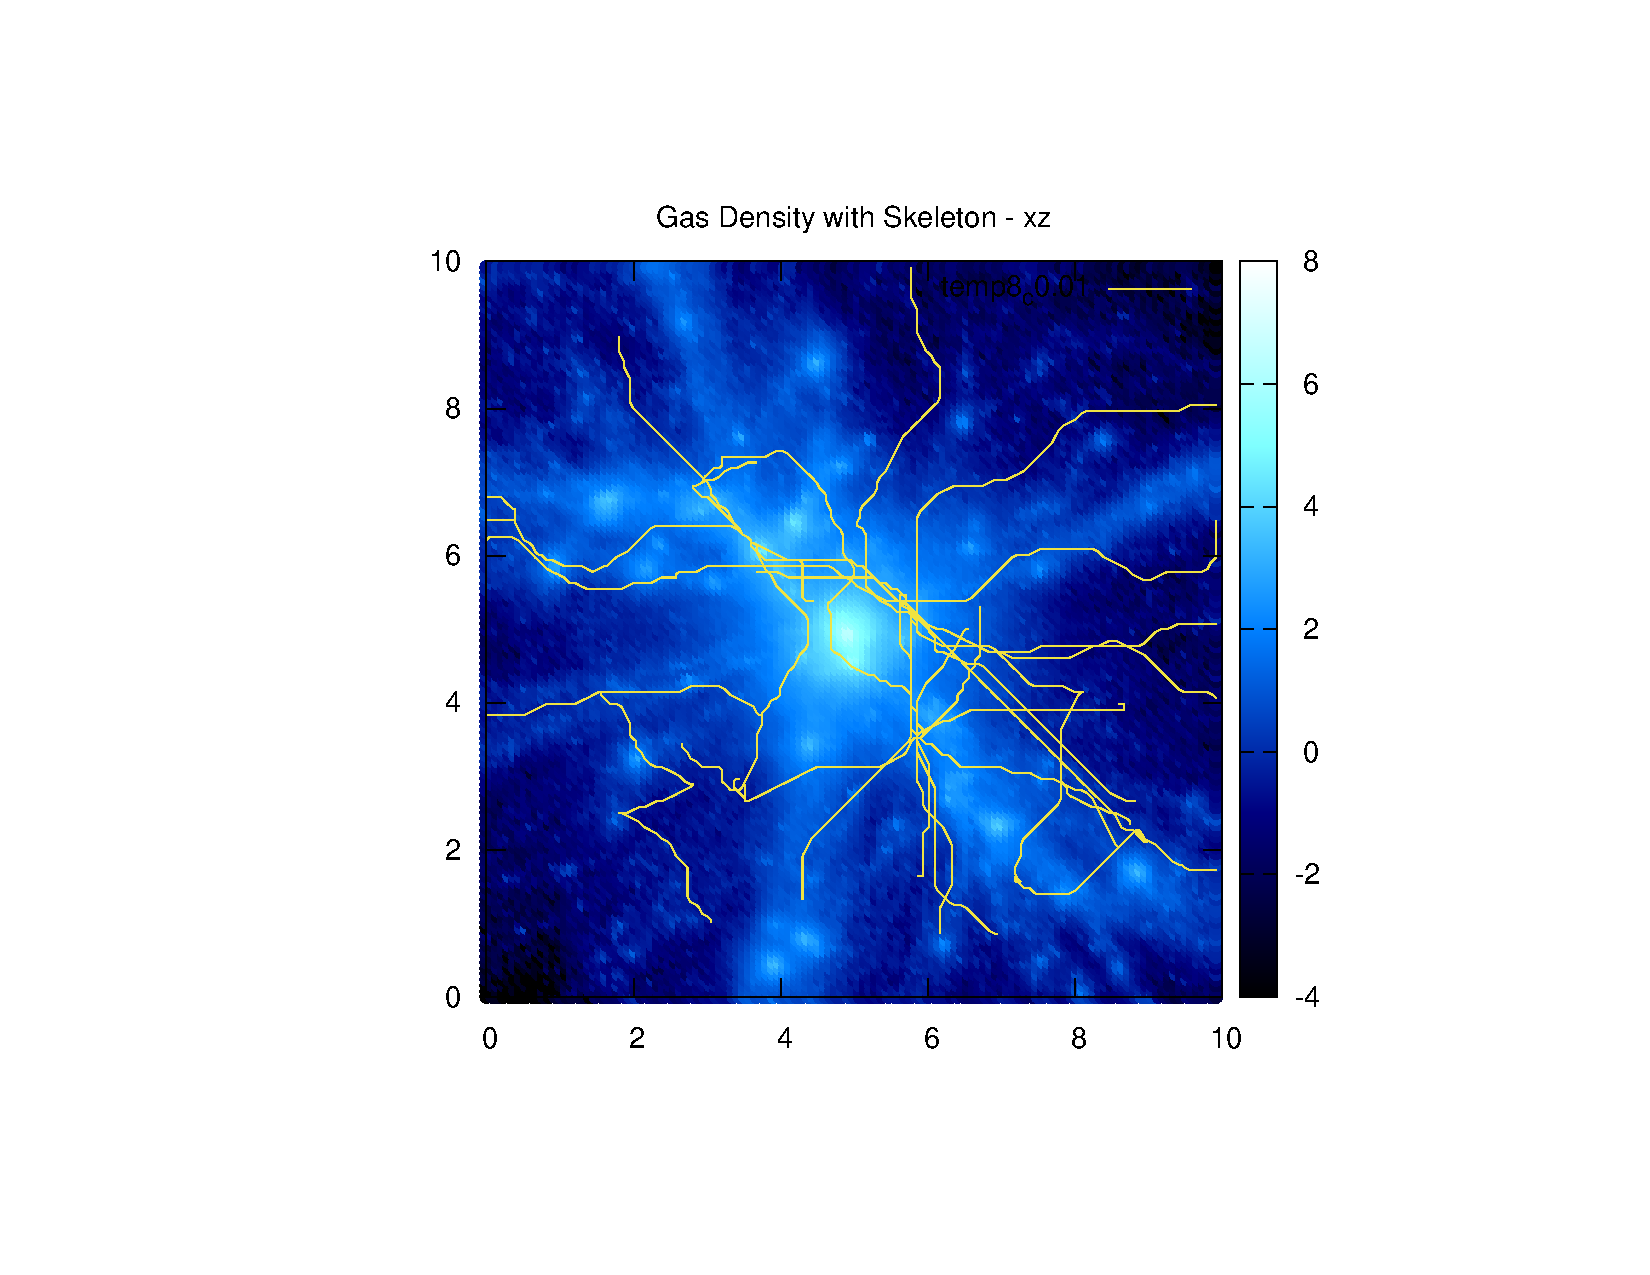
\includegraphics[width=\linewidth]{GasDenSkelxz}
	\end{subfigure}
	\quad
	\begin{subfigure}[t]{0.3\textwidth}
		\centering
		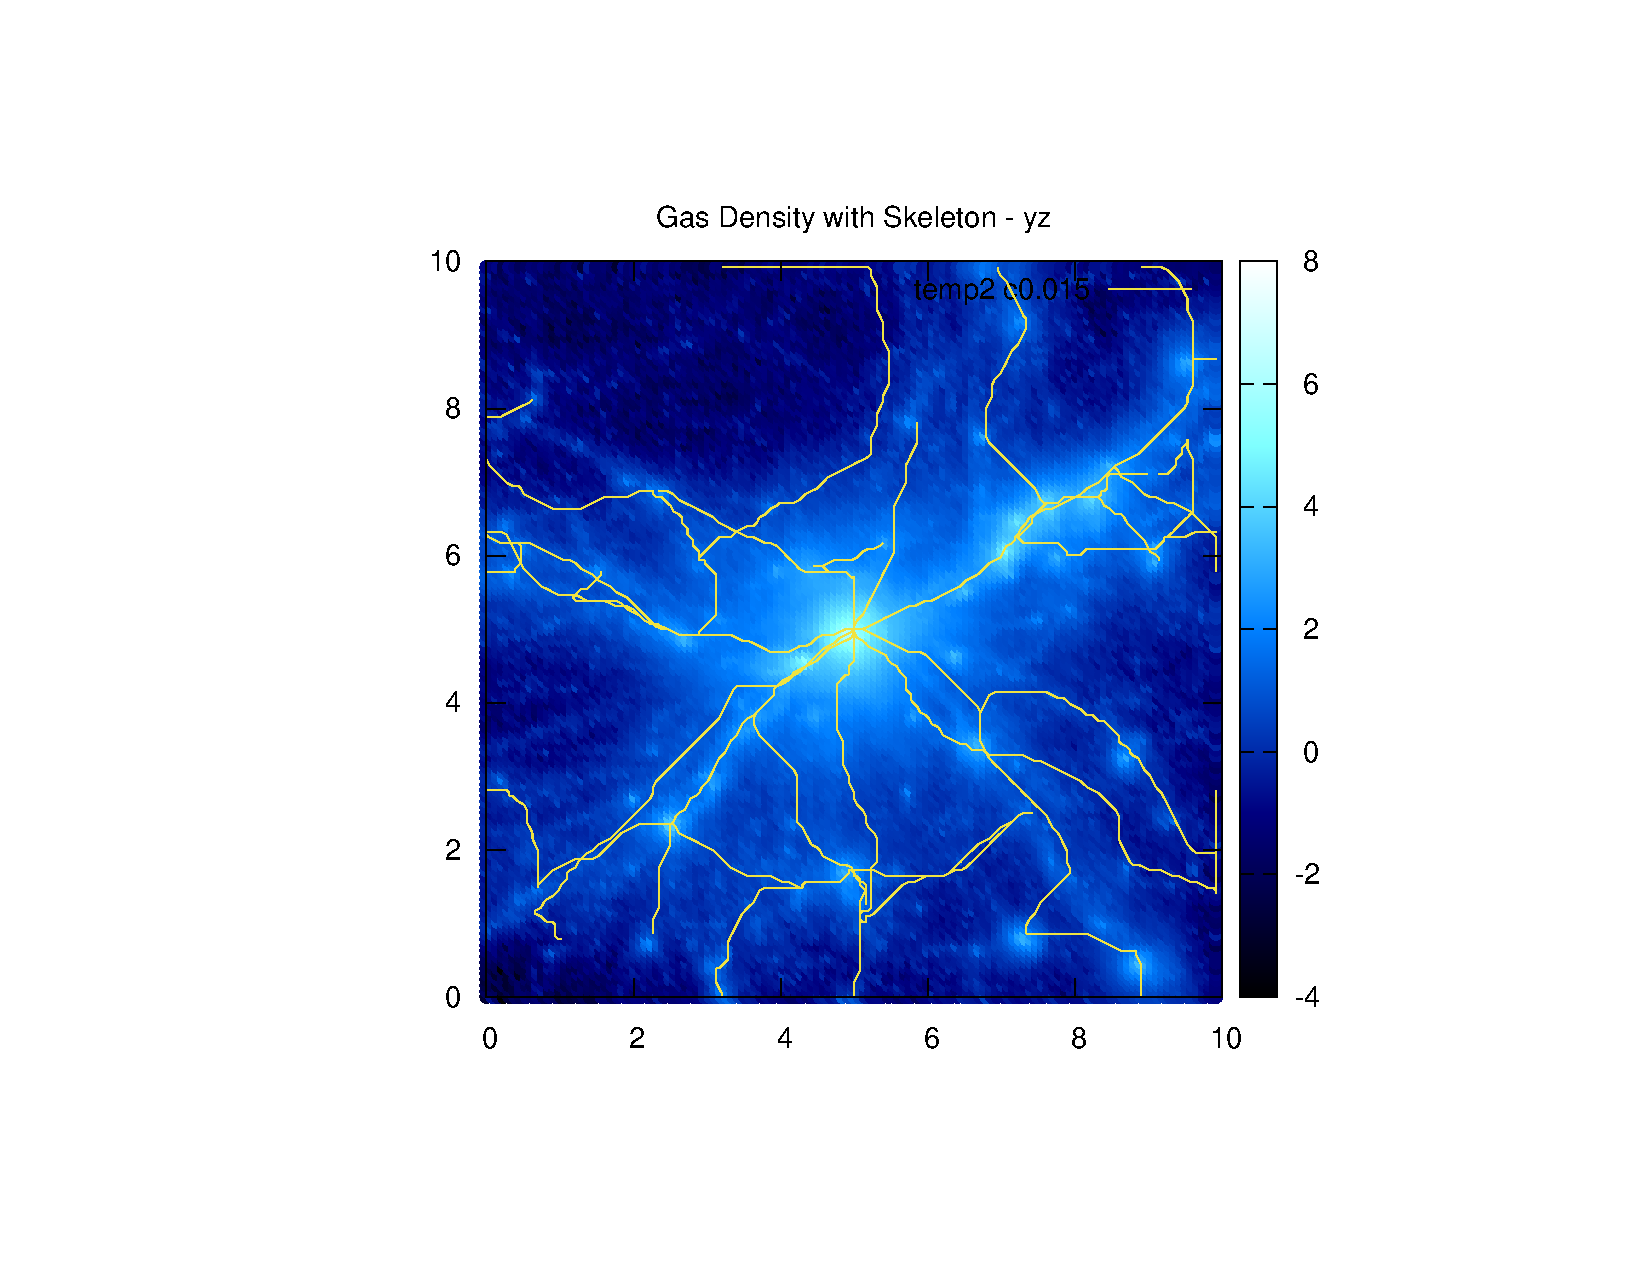
\includegraphics[width=\linewidth]{GasDenSkelyz}
	\end{subfigure}
	\\
	\begin{subfigure}[t]{0.3\textwidth}
		\centering
		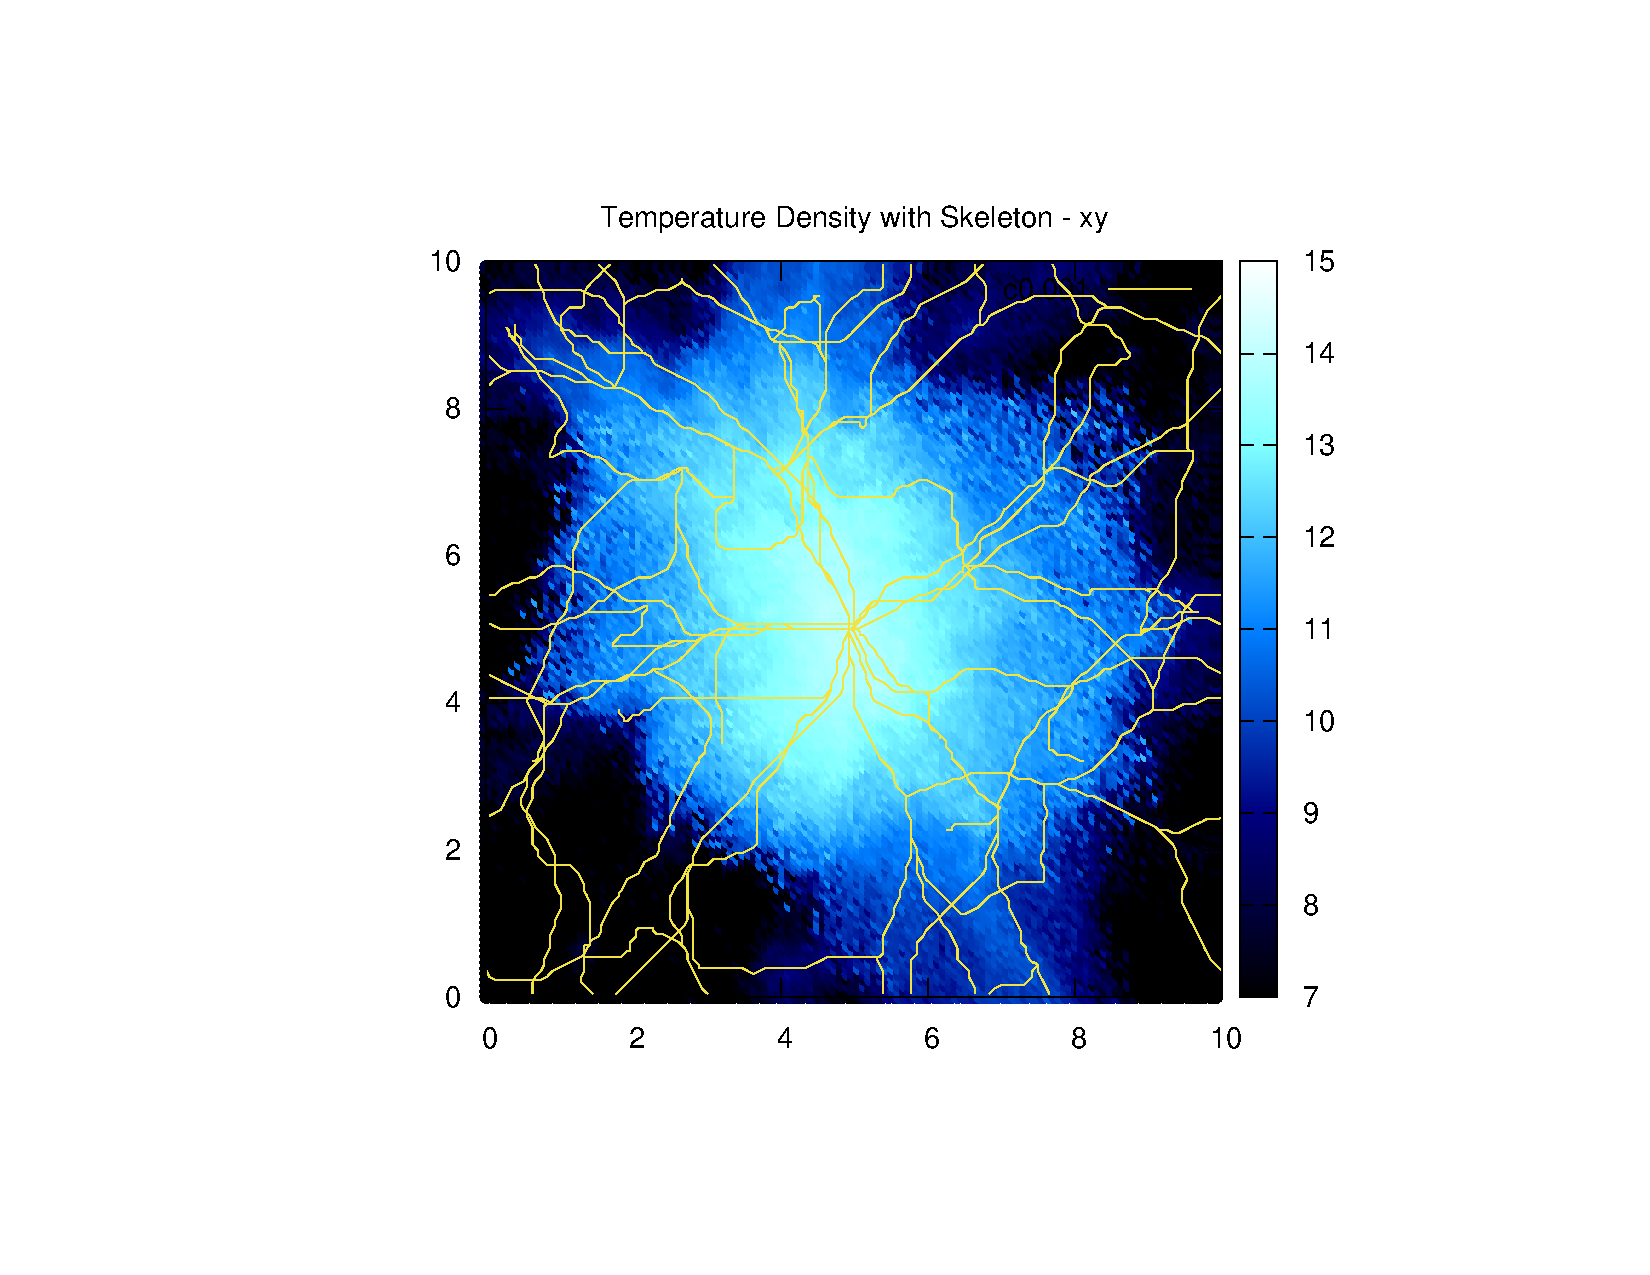
\includegraphics[width=\linewidth]{TempDenSkelxy}
	\end{subfigure}
	\quad
	\begin{subfigure}[t]{0.3\textwidth}
		\centering
		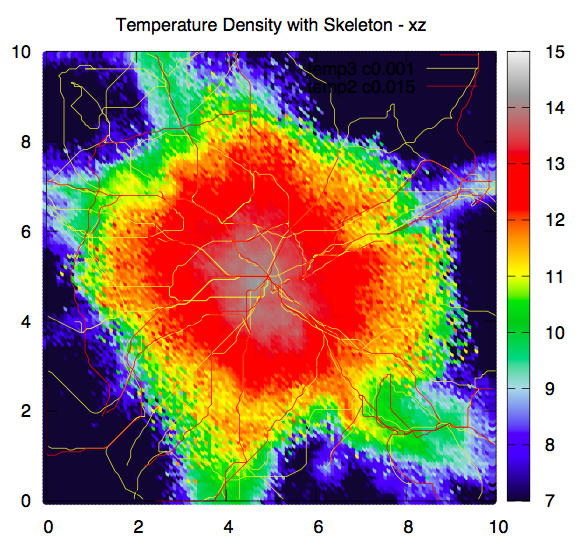
\includegraphics[width=\linewidth]{TempDenSkelxz}
	\end{subfigure}
	\quad
	\begin{subfigure}[t]{0.3\textwidth}
		\centering
		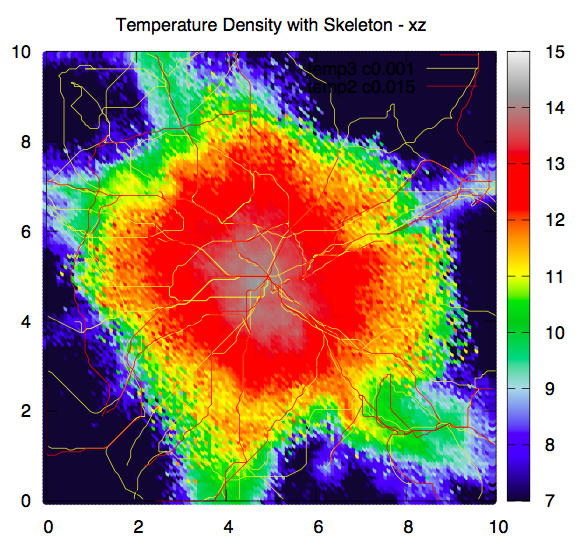
\includegraphics[width=\linewidth]{TempDenSkelxz}
	\end{subfigure}
\label{fig:densities}
\caption{Density plots with overlain skeleton for DM and Gas profiles in xy, xz and yz projections.}
\end{figure*}

%%%%%% METHODS %%%%%
\section{Methodology}
\subsection{Reduced Moment of Inertia Tensor}
The physical shape characteristics of the stellar halo can be calculated in a number of different ways, all of which influence the resulting correlations made with the background filament. An important quantity for characterising shape is the moment of inertia tensor, which can be calculated iteratively for a set of particles as per Porciani \cite{porciani02a}. A more useful version is the reduced moment of inertia tensor \cite{tenneti15} which produces a direct correlation between eigenvalues and the principle axes of the assumed elliptic halo. The reduced inertia tensor was calculated for each halo cube according to the following equation:
\begin{equation}
	\tilde{I}_{ij}=\frac{\sum_n m_n \frac{x_{ni}x_{nj}}{r^2_n}}{\sum_n m_n}, \quad \quad \text{where} \quad r^2_n=\sum_i x^2_{ni}
	\label{eq:moitensor}
\end{equation}
Where the generalised $x_i$ coordinates are given with respect to the centre of mass of the halo, which was calculated iteratively for circles of increasingly smaller radii. From this reduced inertia tensor, the eigenvectors represent the principal axes of the halo ellipsoid, and the eigenvalues correspond to the square of the principal axes' lengths. That is, for eigenvalues $\lambda_{a} \geq \lambda_{b} \geq \lambda_{c} $ the lengths of the major, intermediate and minor axes $l_{a},l_{b},l_{c}$ are then $\sqrt{\lambda_{a}}, \sqrt{\lambda_{b}}, \sqrt{\lambda_{c}}$. Note that this only holds because the reduced moment of inertia tensor was calculated.
Since the reduced moment of inertia tensor produces a real symmetric matrix, the eigenvalues and eigenvectors were calculated analytically. 

\begin{figure*}[!t]
\centering
	\begin{subfigure}[t]{0.3\textwidth}
		\centering
		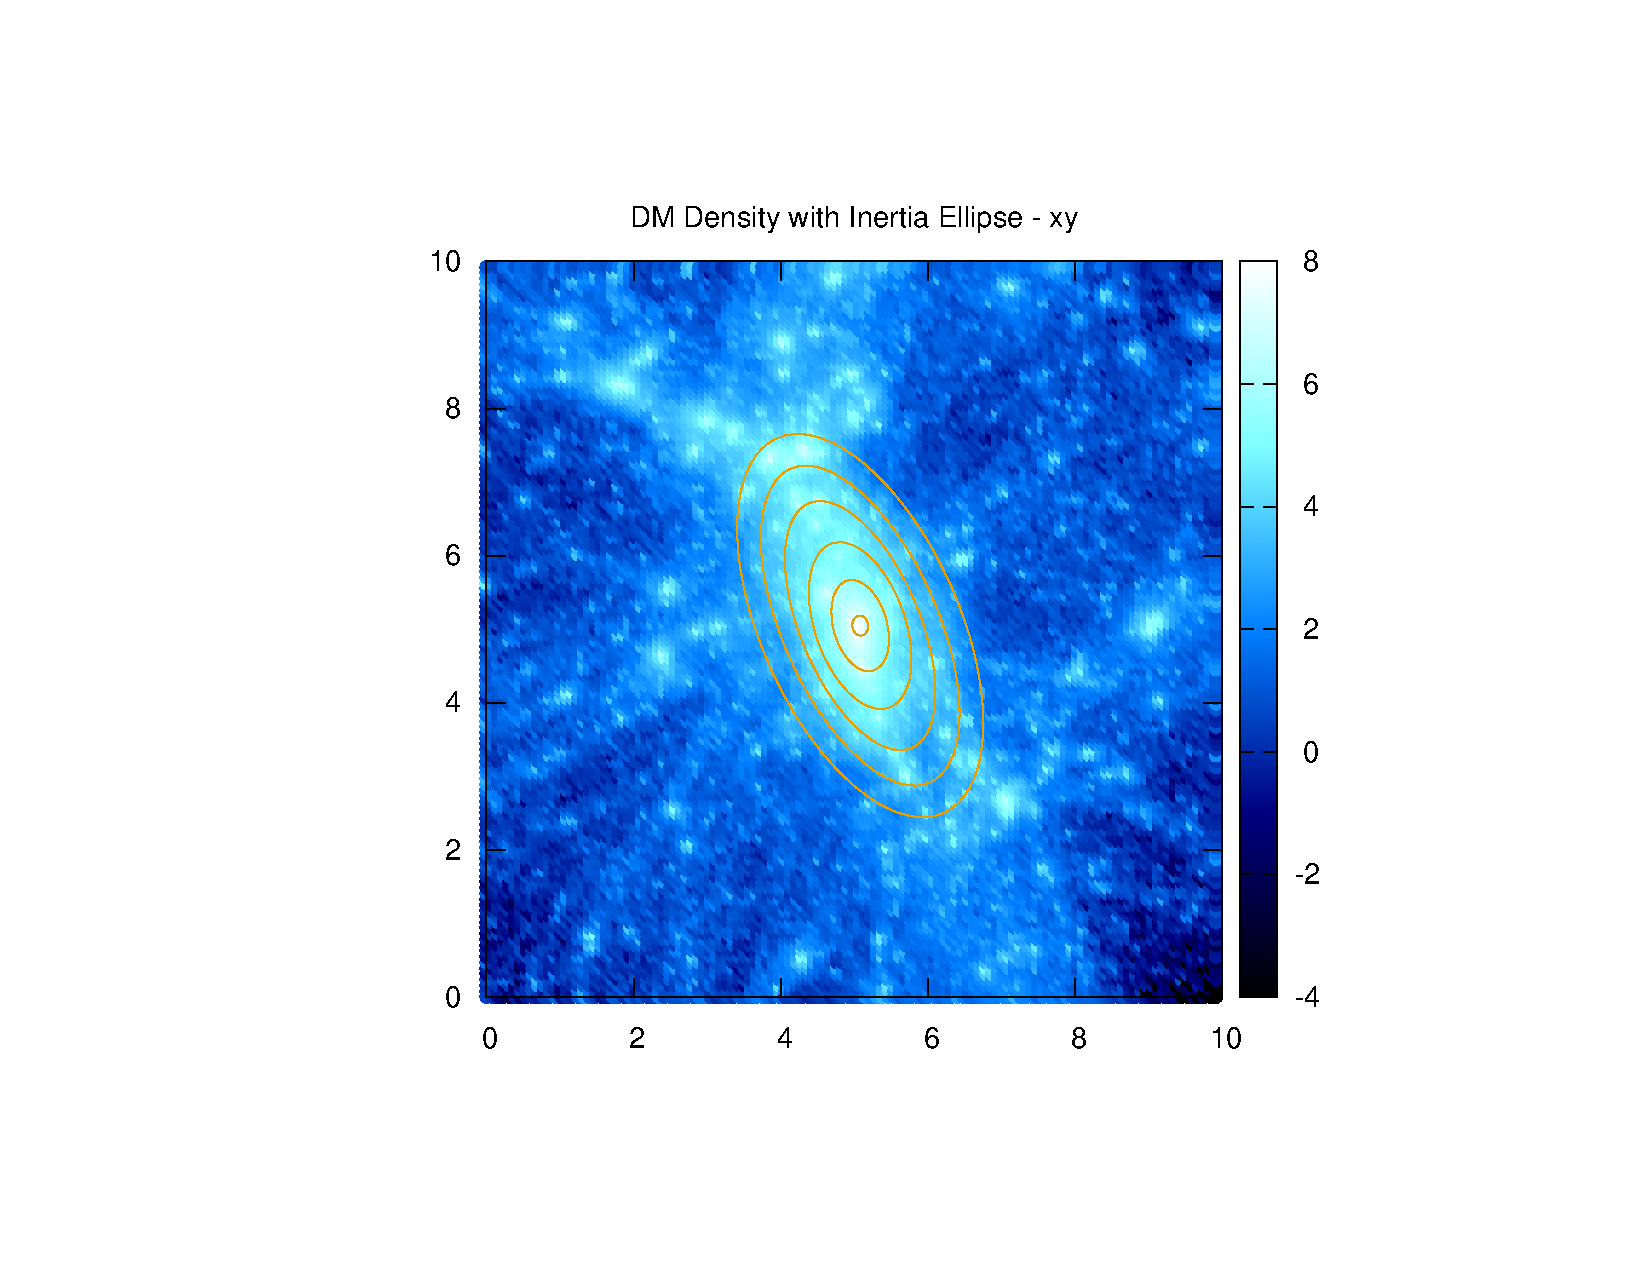
\includegraphics[width=\linewidth]{DMDenEllipxy}
	\end{subfigure}
	\quad
	\begin{subfigure}[t]{0.3\textwidth}
		\centering
		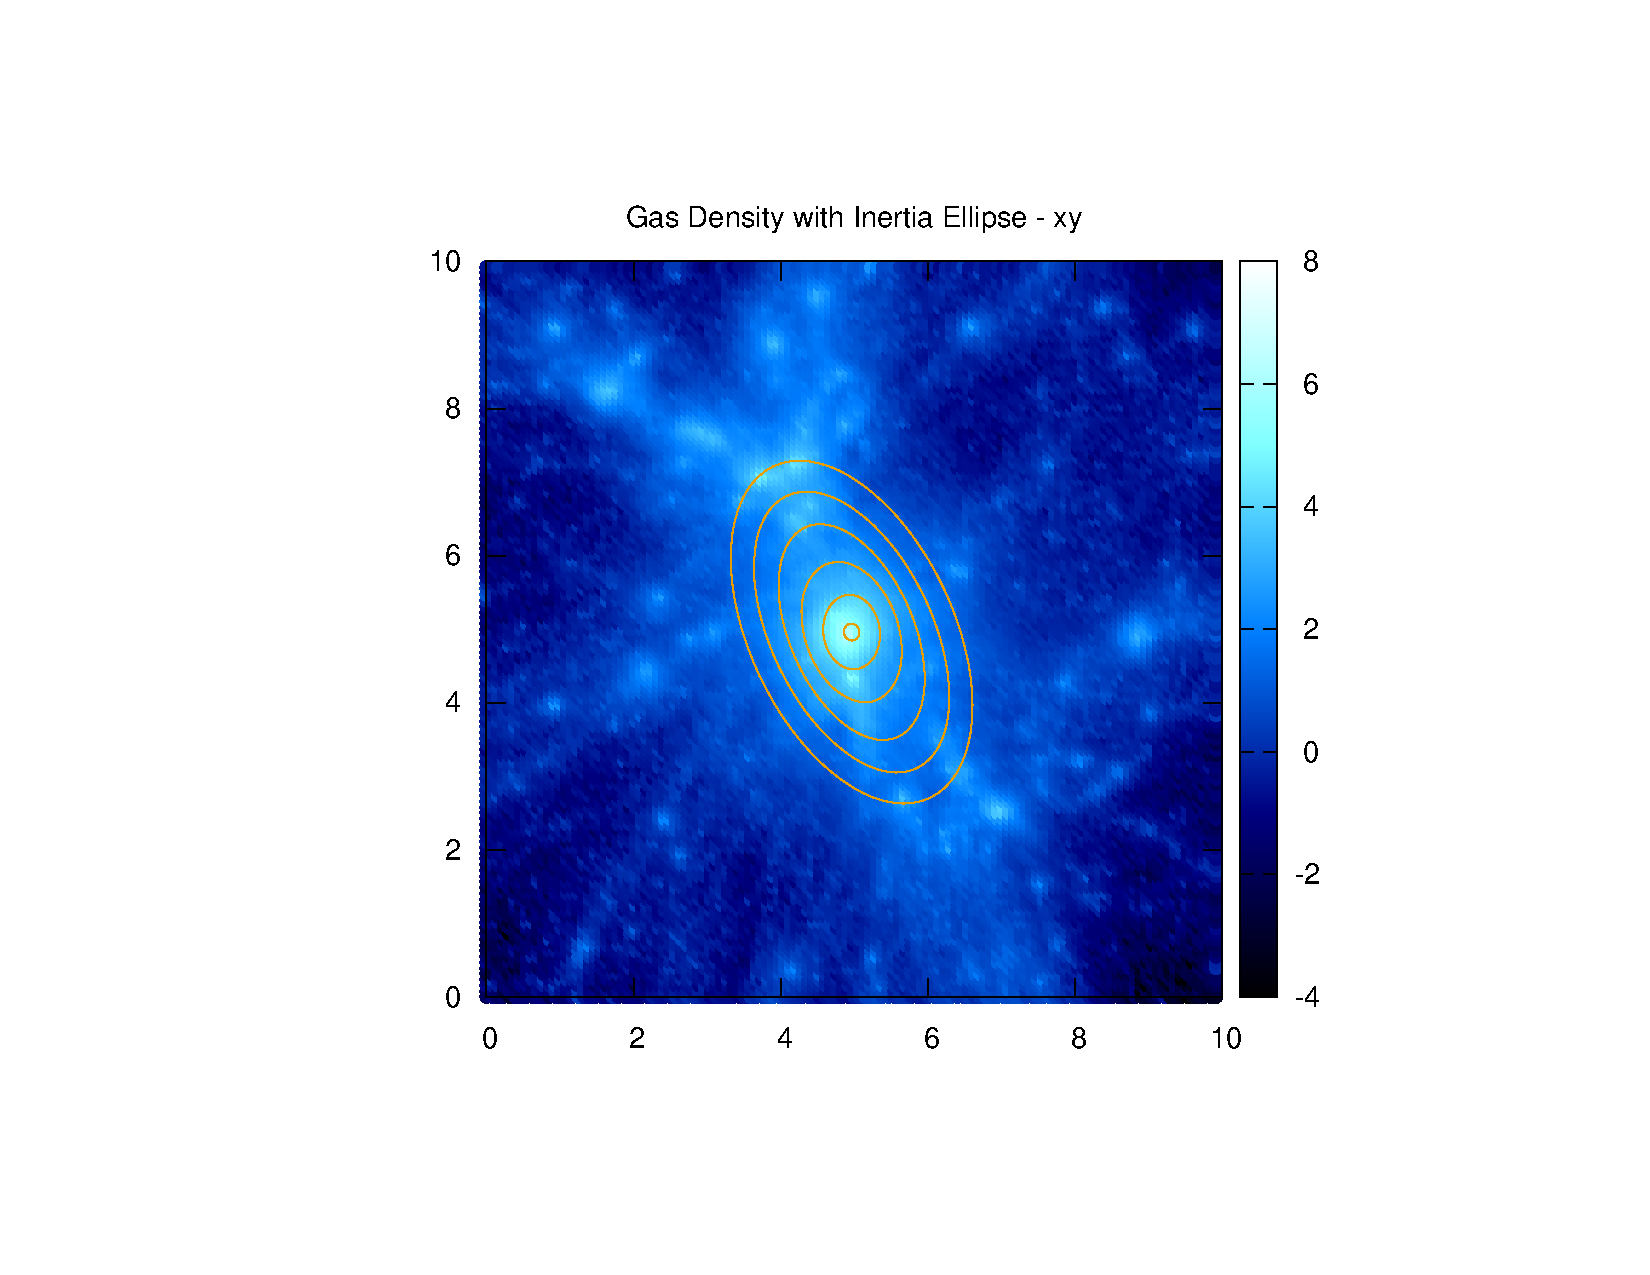
\includegraphics[width=\linewidth]{GasDenEllipxy}
	\end{subfigure}
	\quad
	\begin{subfigure}[t]{0.3\textwidth}
		\centering
		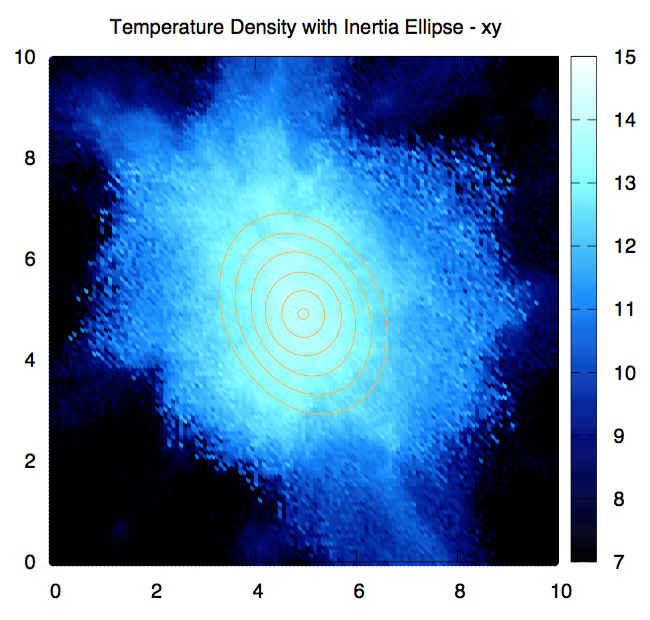
\includegraphics[width=\linewidth]{TempDenEllipxy}
	\end{subfigure}
	\\
	\begin{subfigure}[t]{0.3\textwidth}
		\centering
		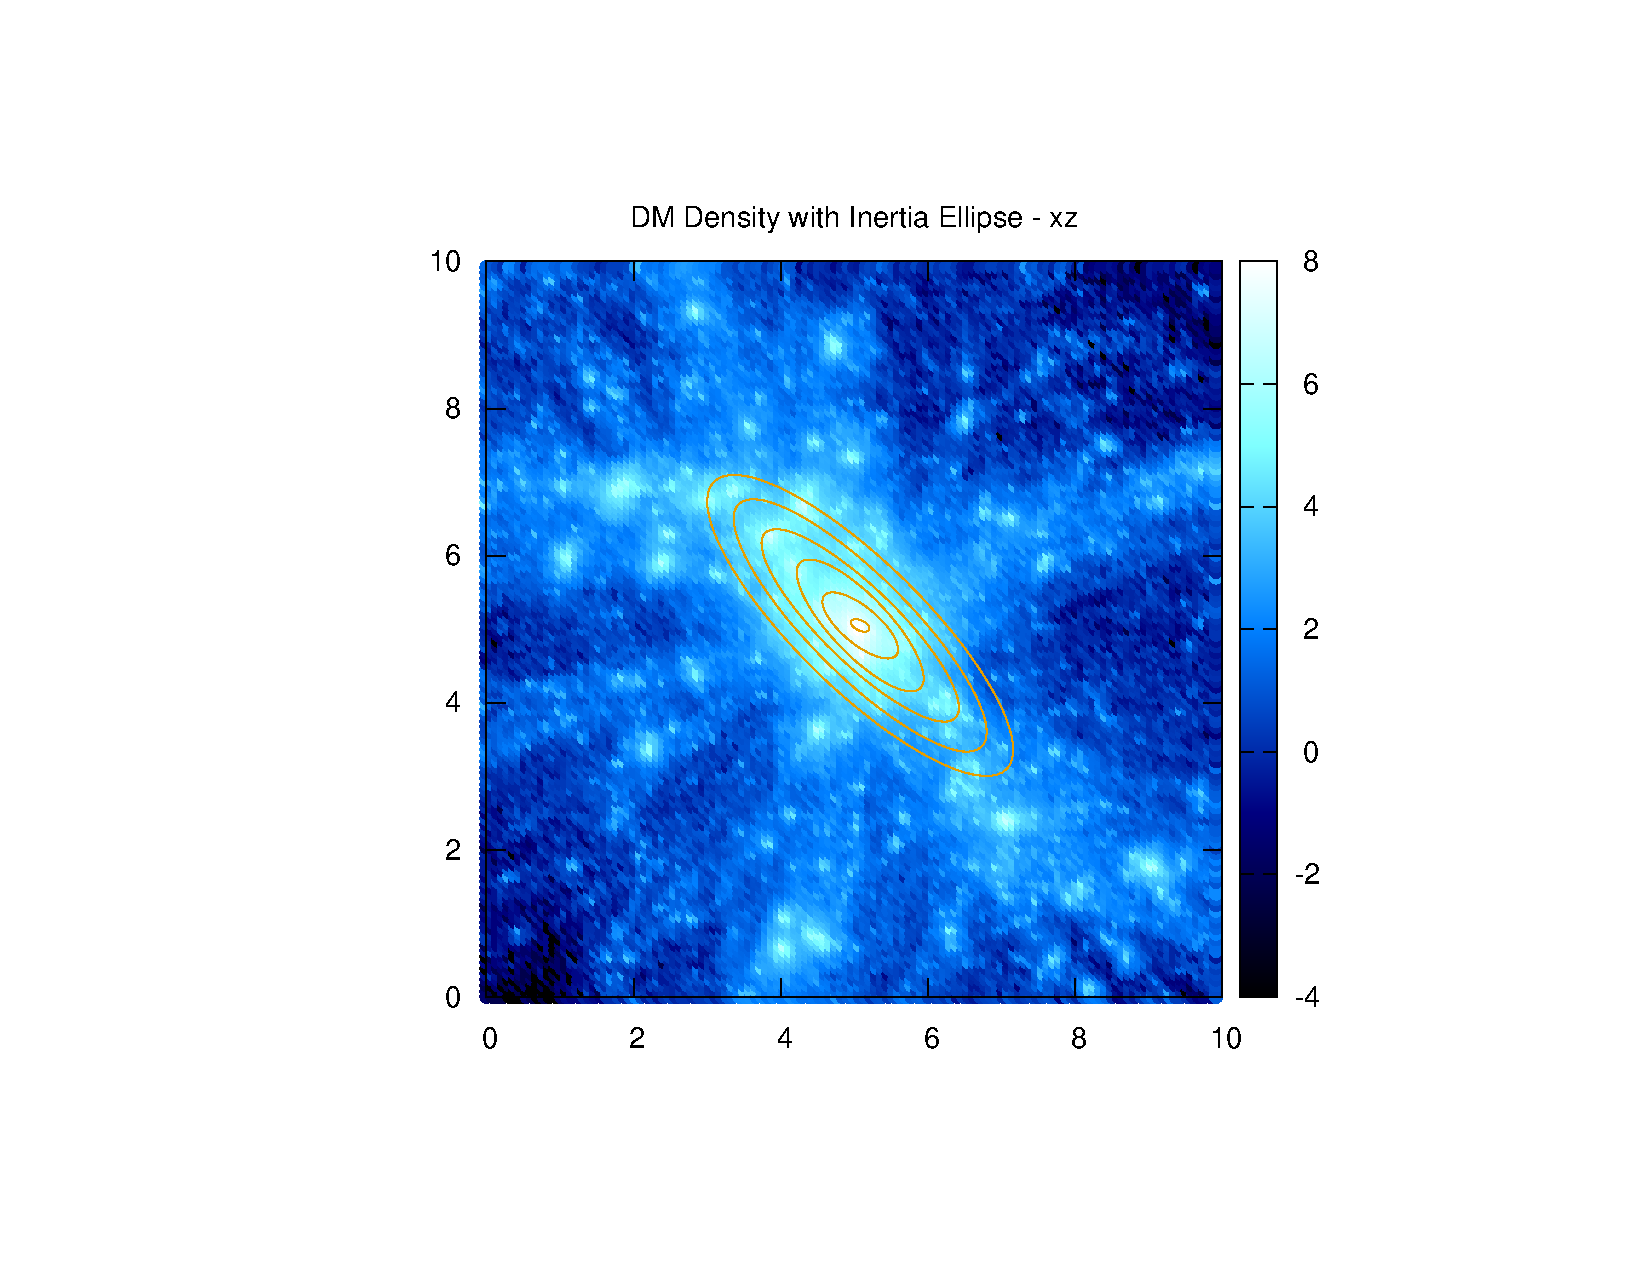
\includegraphics[width=\linewidth]{DMDenEllipxz}
	\end{subfigure}
	\quad
	\begin{subfigure}[t]{0.3\textwidth}
		\centering
		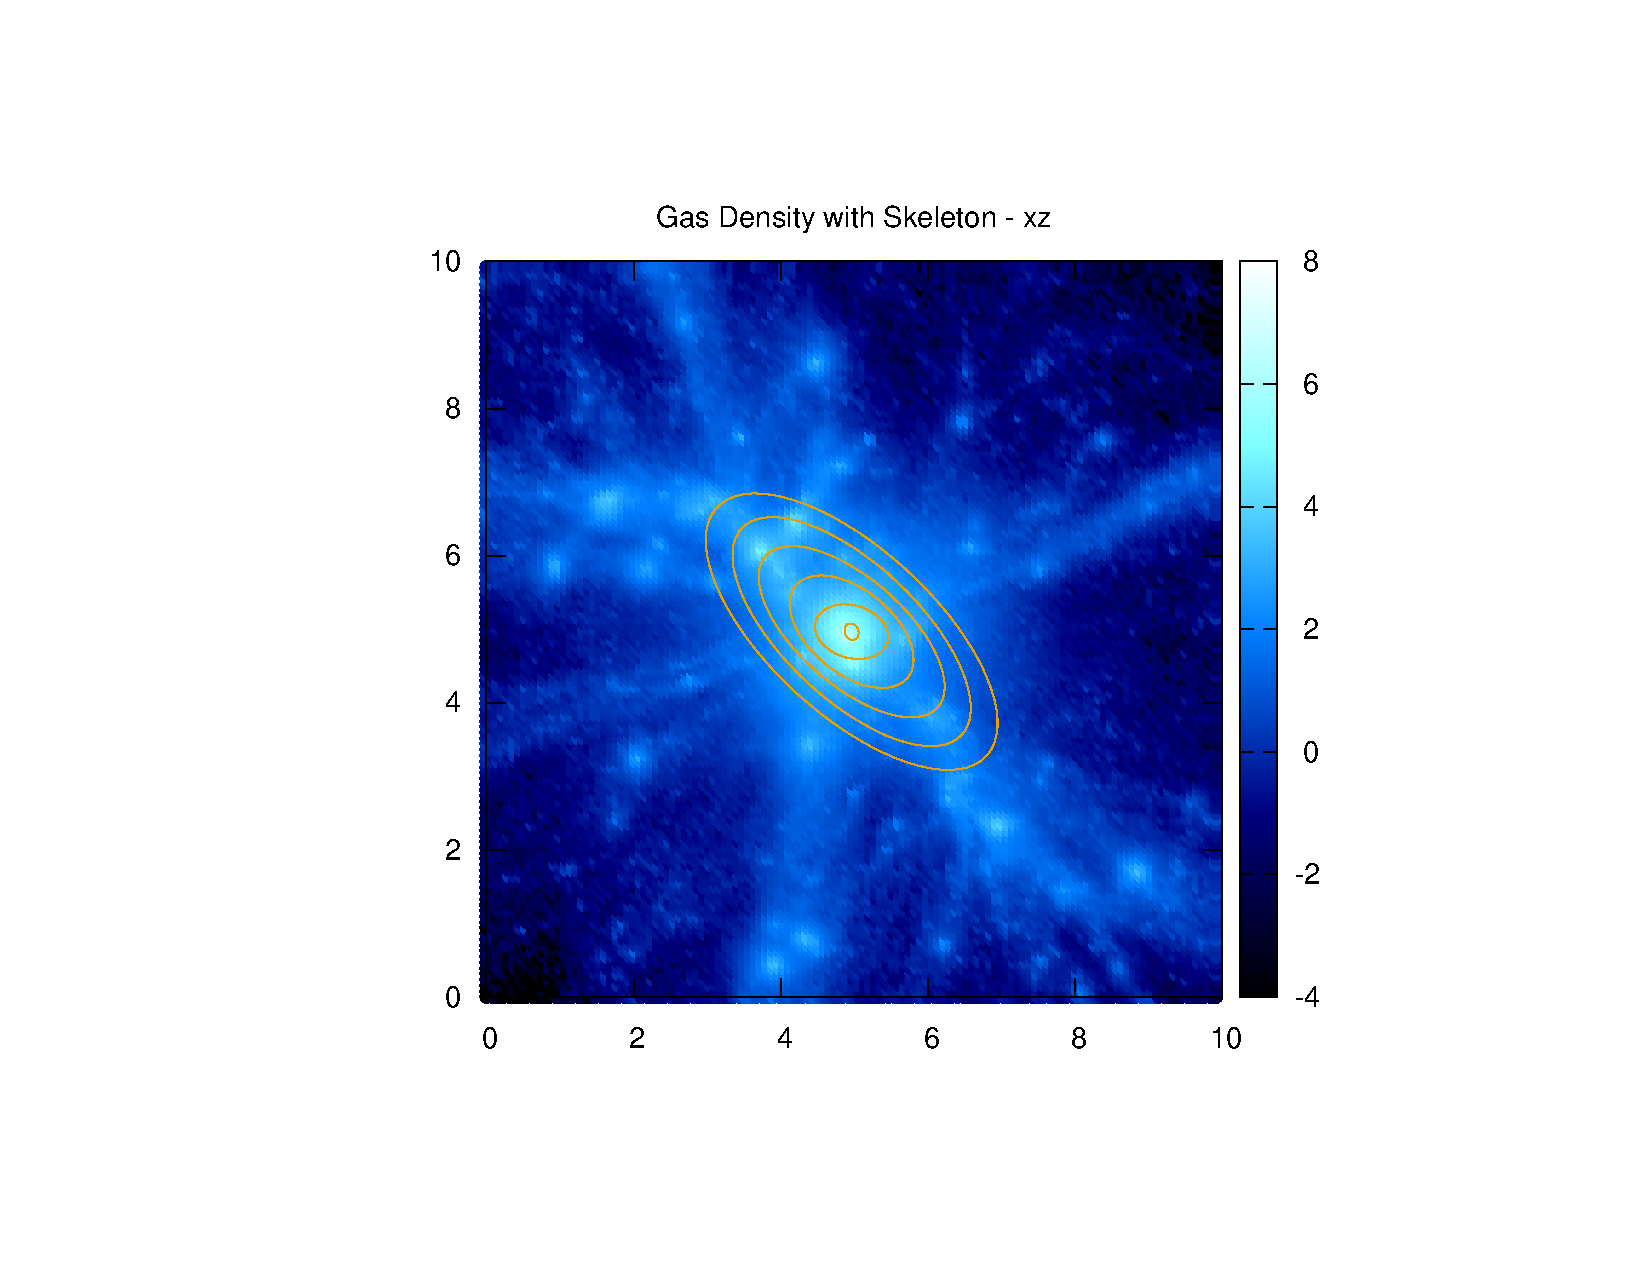
\includegraphics[width=\linewidth]{GasDenEllipxz}
	\end{subfigure}
	\quad
	\begin{subfigure}[t]{0.3\textwidth}
		\centering
		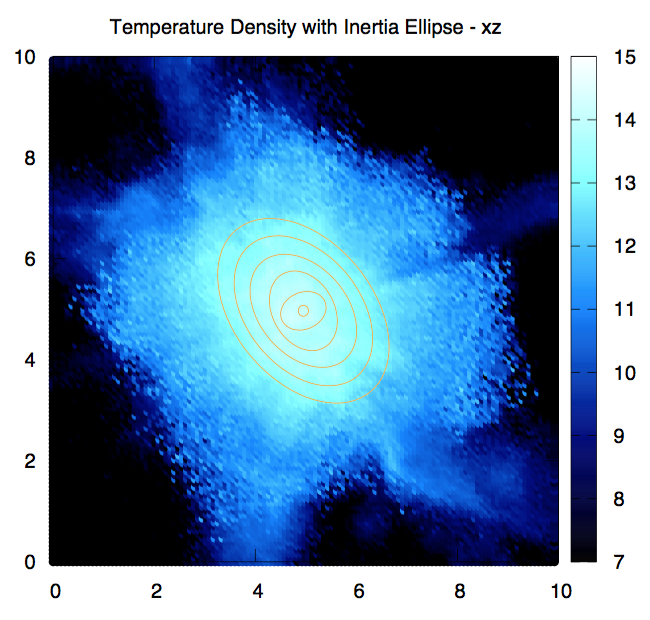
\includegraphics[width=\linewidth]{TempDenEllipxz}
	\end{subfigure}
	\\
	\begin{subfigure}[t]{0.3\textwidth}
		\centering
		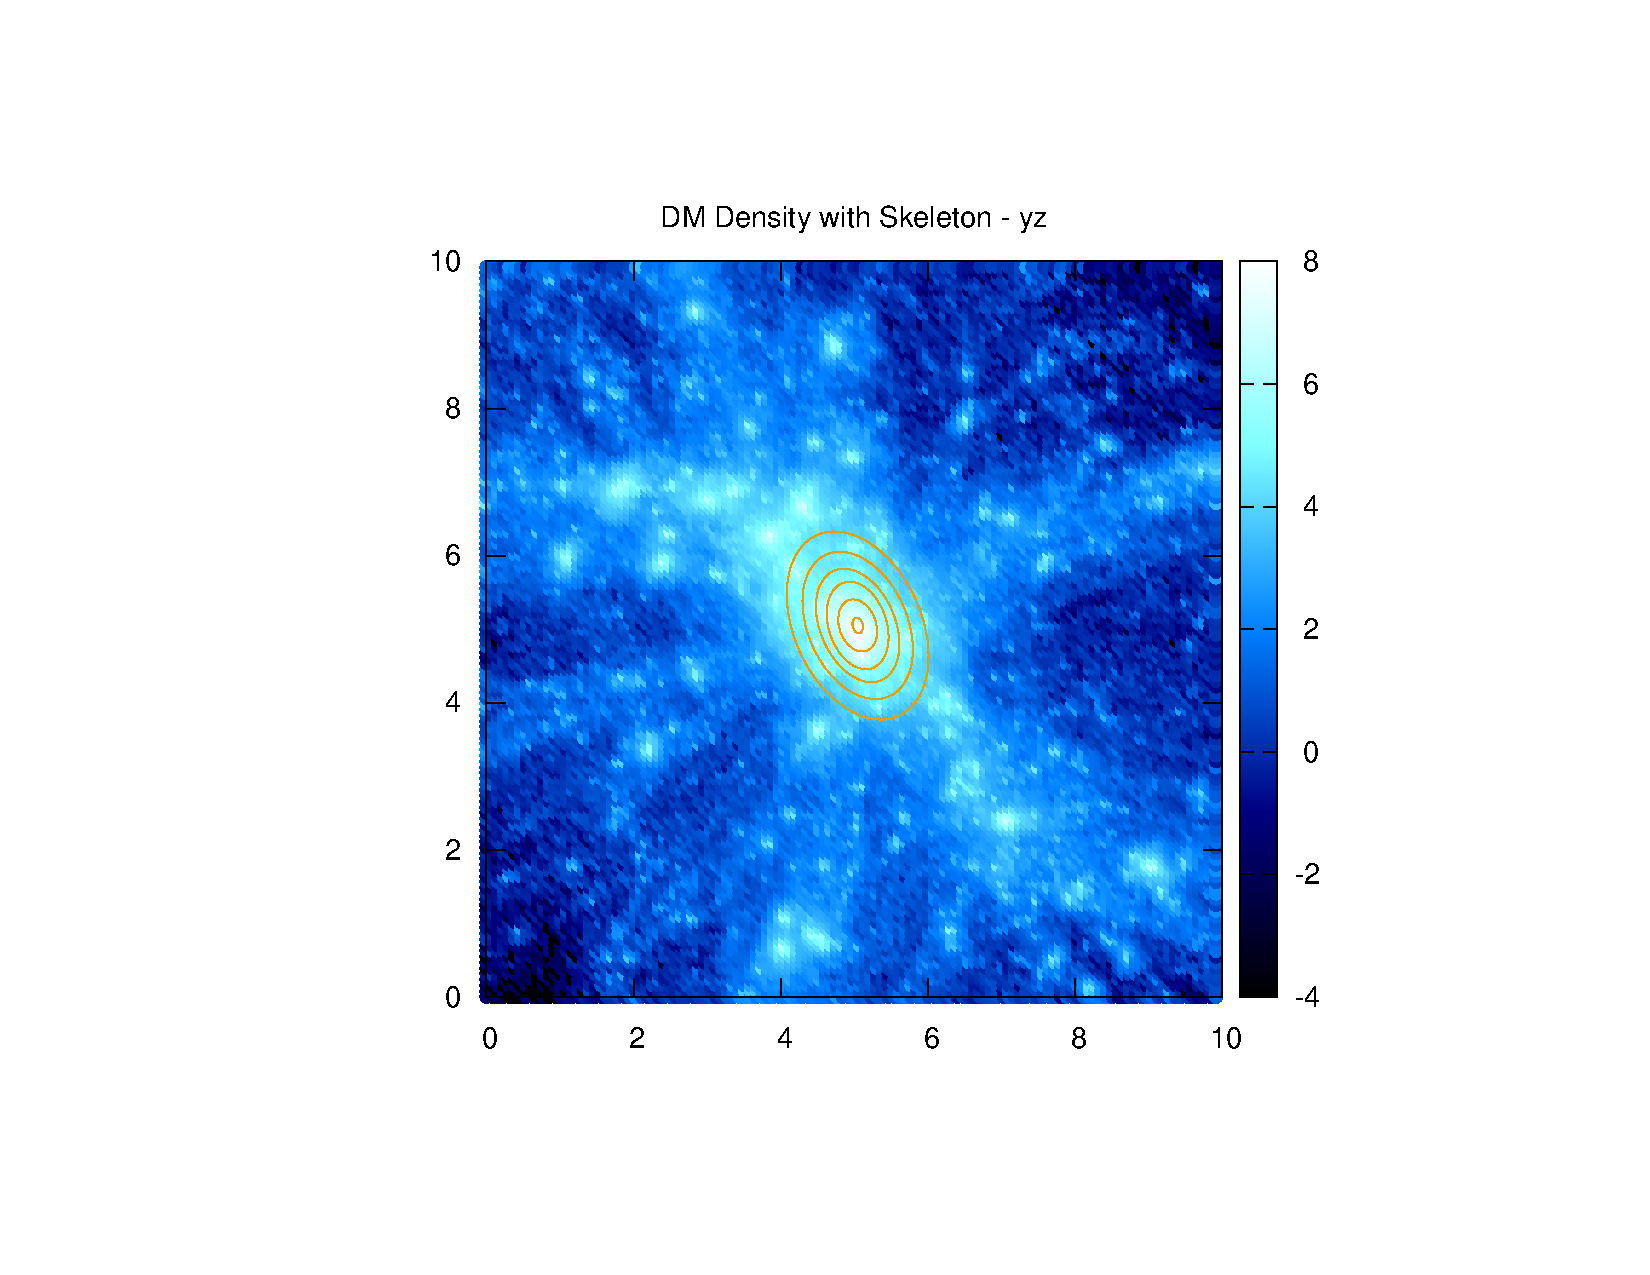
\includegraphics[width=\linewidth]{DMDenEllipyz}
	\end{subfigure}
	\quad
	\begin{subfigure}[t]{0.3\textwidth}
		\centering
		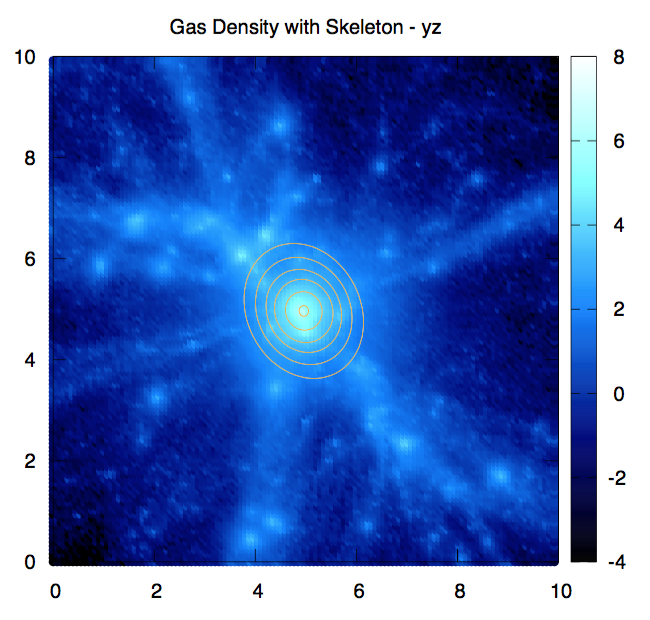
\includegraphics[width=\linewidth]{GasDenEllipyz}
	\end{subfigure}
	\quad
	\begin{subfigure}[t]{0.3\textwidth}
		\centering
		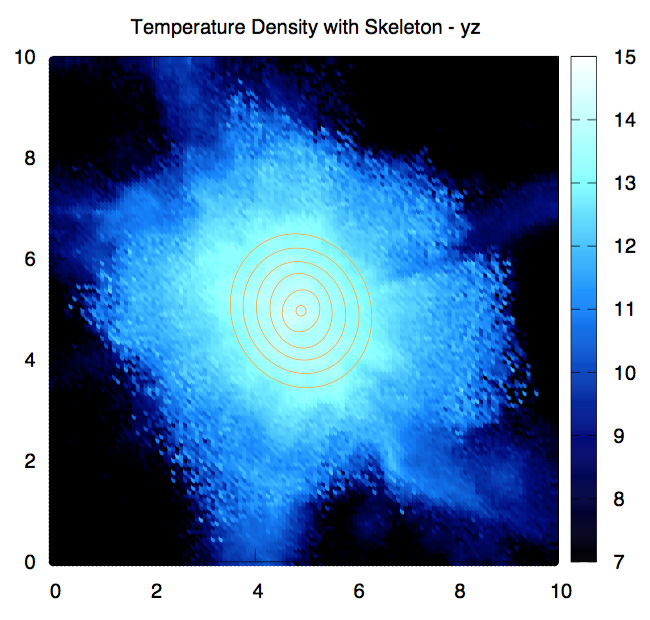
\includegraphics[width=\linewidth]{TempDenEllipyz}
	\end{subfigure}
\label{fig:ellipses}
\caption{Ellipses in xy projection for reduced moment of inertia tensor eigenvectors for a) DM, b) stellar matter and c) temperature.}
\end{figure*}

\subsection{Shape Properties of Stellar Halos}
Using the values for the major, intermediate and minor axes of the elliptic halo, and their corresponding axis vectors, the following quantities were measured. 
\IEEEPARstart{}{Sphericity}: The sphericity of the object is defined with respect to the major and minor axis (the intermediate is ignored). Plotting the sphericity of the stellar and dark matter halo as a function of radius gives an insight into the elongating effects of matter inflow along the filament, and to what extent the halos hold their shape under this force. A spherical halo has sphericity $S=1$ whereas a needle would have $S=0$ \cite{hahn07a}.
\IEEEPARstart{}{Triaxiality}: The triaxiality of the object takes into account all three axes. A prolate halo, one which is lengthened in the direction of its poles, has $T=1$ and an oblate (flattened at the poles) will have $T=0$ \cite{hahn07a}.
\begin{equation}
	S=\frac{l_c}{l_a}, \quad \quad T=\frac{l_a^2-l_b^2}{l_a^2-l_c^2}
	\label{eq:sph&tri}
\end{equation}
\IEEEPARstart{}{Ellipticity}: Perhaps the most significant quantity in regards to this analysis however is the ellipticity, calculated using again only the major and minor axes of the halo. The significance of this comes from the fact the reduced moment of inertia tensor is calculated assuming an ellipsoid body. The ellipticity also gives a measure of how much the halo has been flattened along the filament, ignoring effects of the intermediate axis. The halo would be expected to have more prolate at higher radii as matter streams along the filament to the node.
\begin{equation}
	E=\sqrt{\frac{l_a^2-l_c^2}{l_a^2}}
	\label{eq:ellipticity}
\end{equation}

\begin{figure*}[!t]
\centering
	\begin{subfigure}[t]{0.3\textwidth}
		\centering
		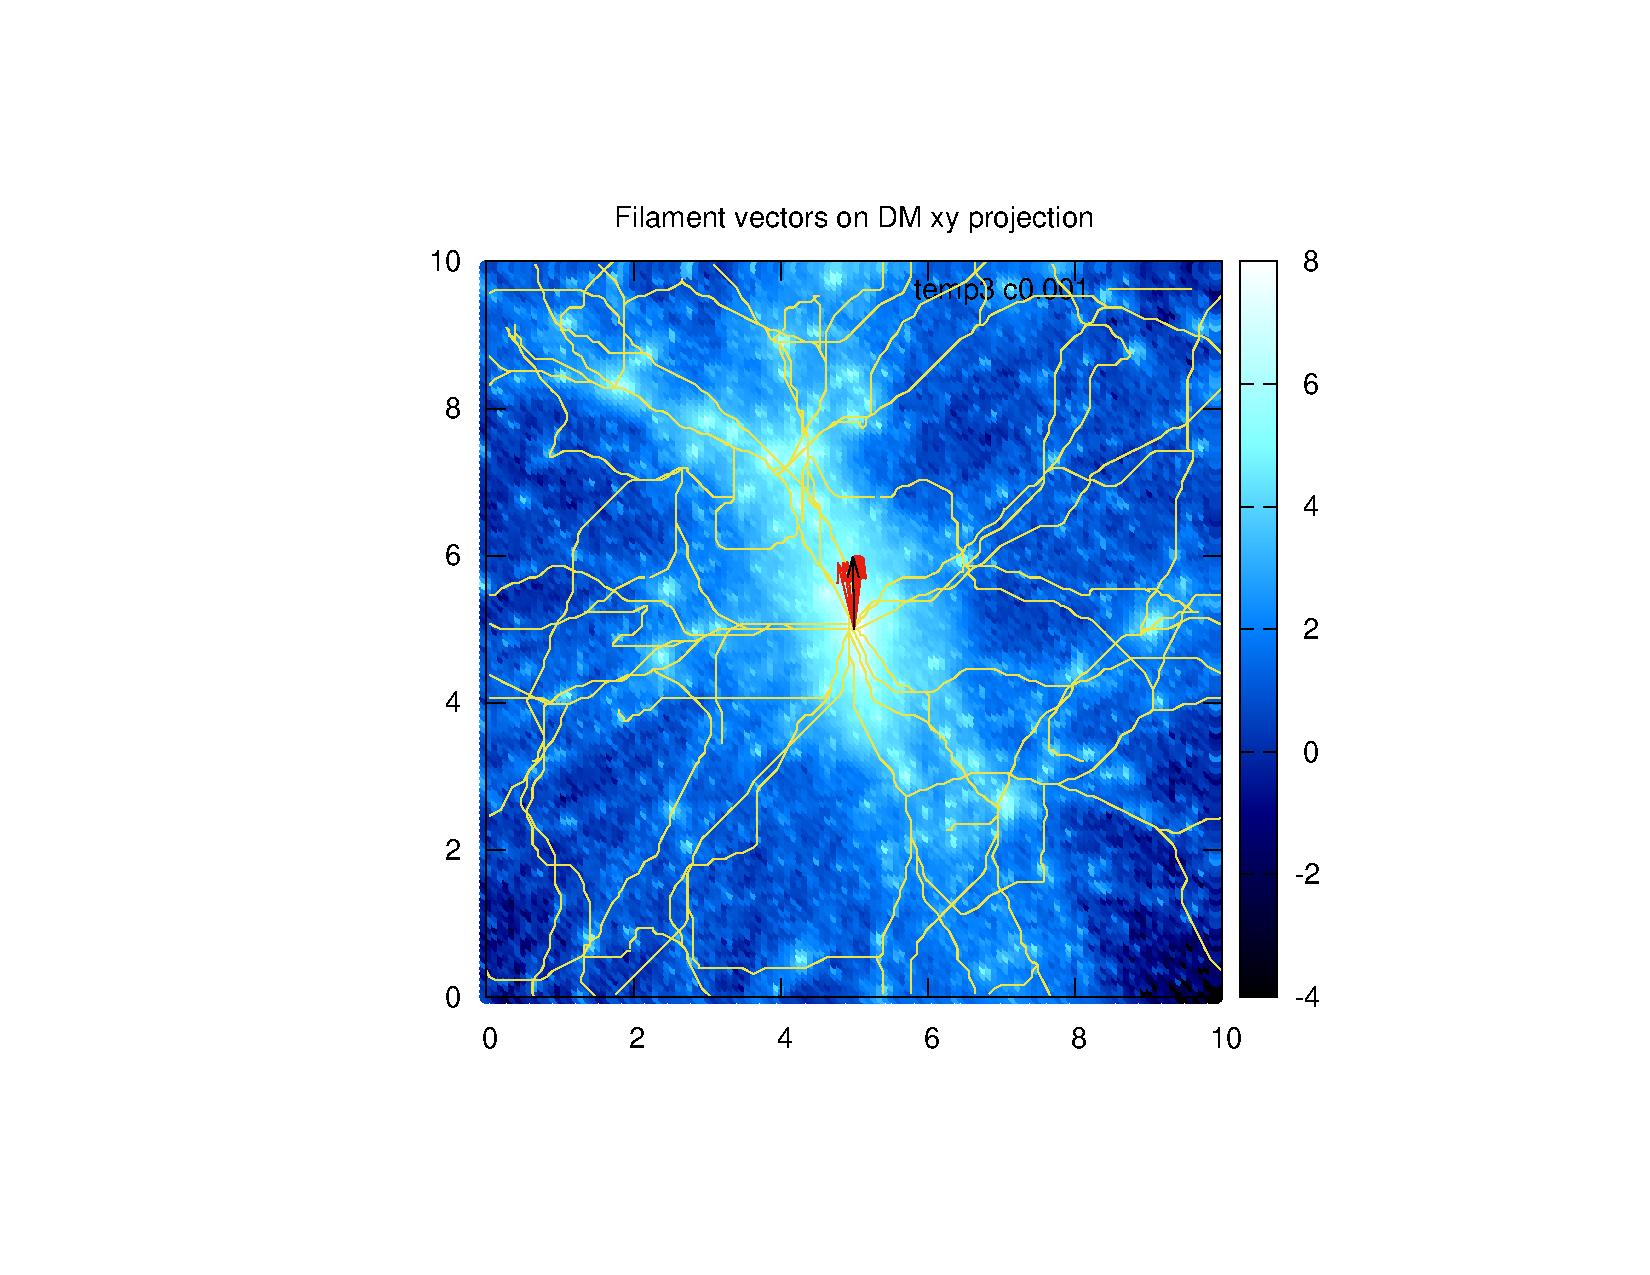
\includegraphics[width=\linewidth]{FilxyDM}
	\end{subfigure}
	\quad
	\begin{subfigure}[t]{0.3\textwidth}
		\centering
		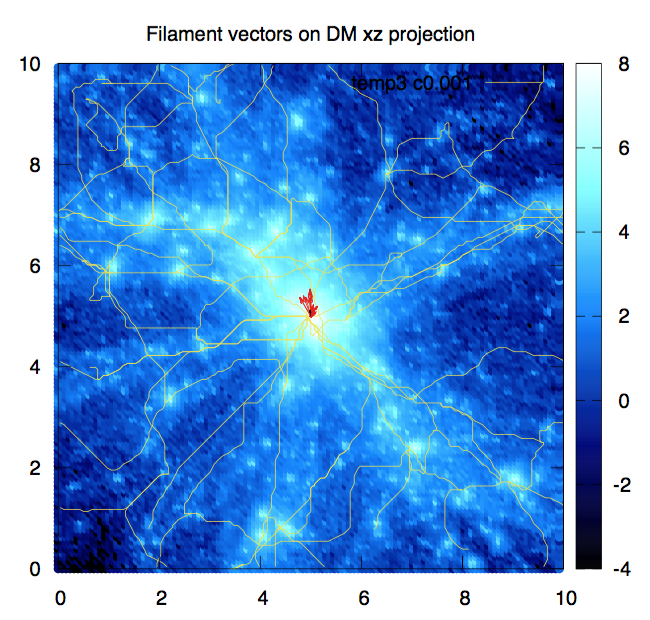
\includegraphics[width=\linewidth]{FilxzDM}
	\end{subfigure}
	\quad
	\begin{subfigure}[t]{0.3\textwidth}
		\centering
		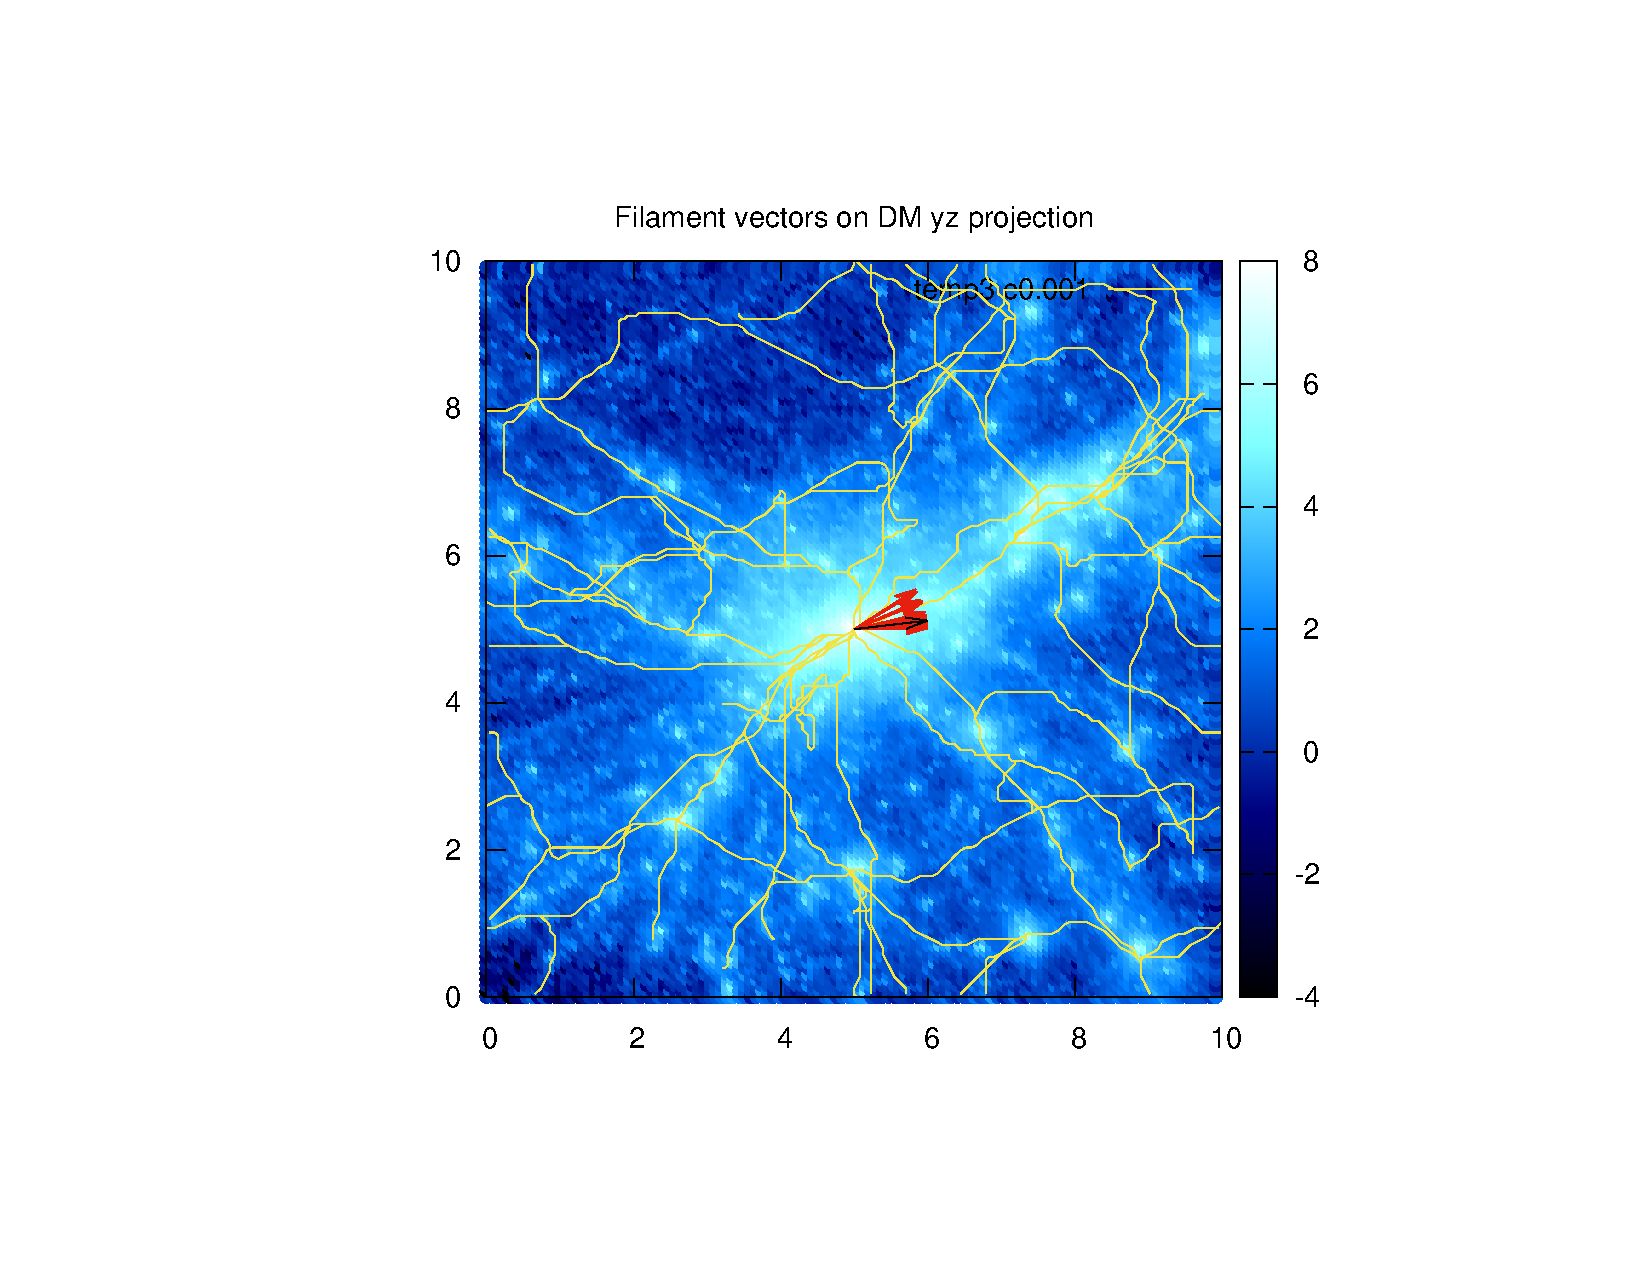
\includegraphics[width=\linewidth]{FilyzDM}
	\end{subfigure}
	\\
	\begin{subfigure}[t]{0.3\textwidth}
		\centering
		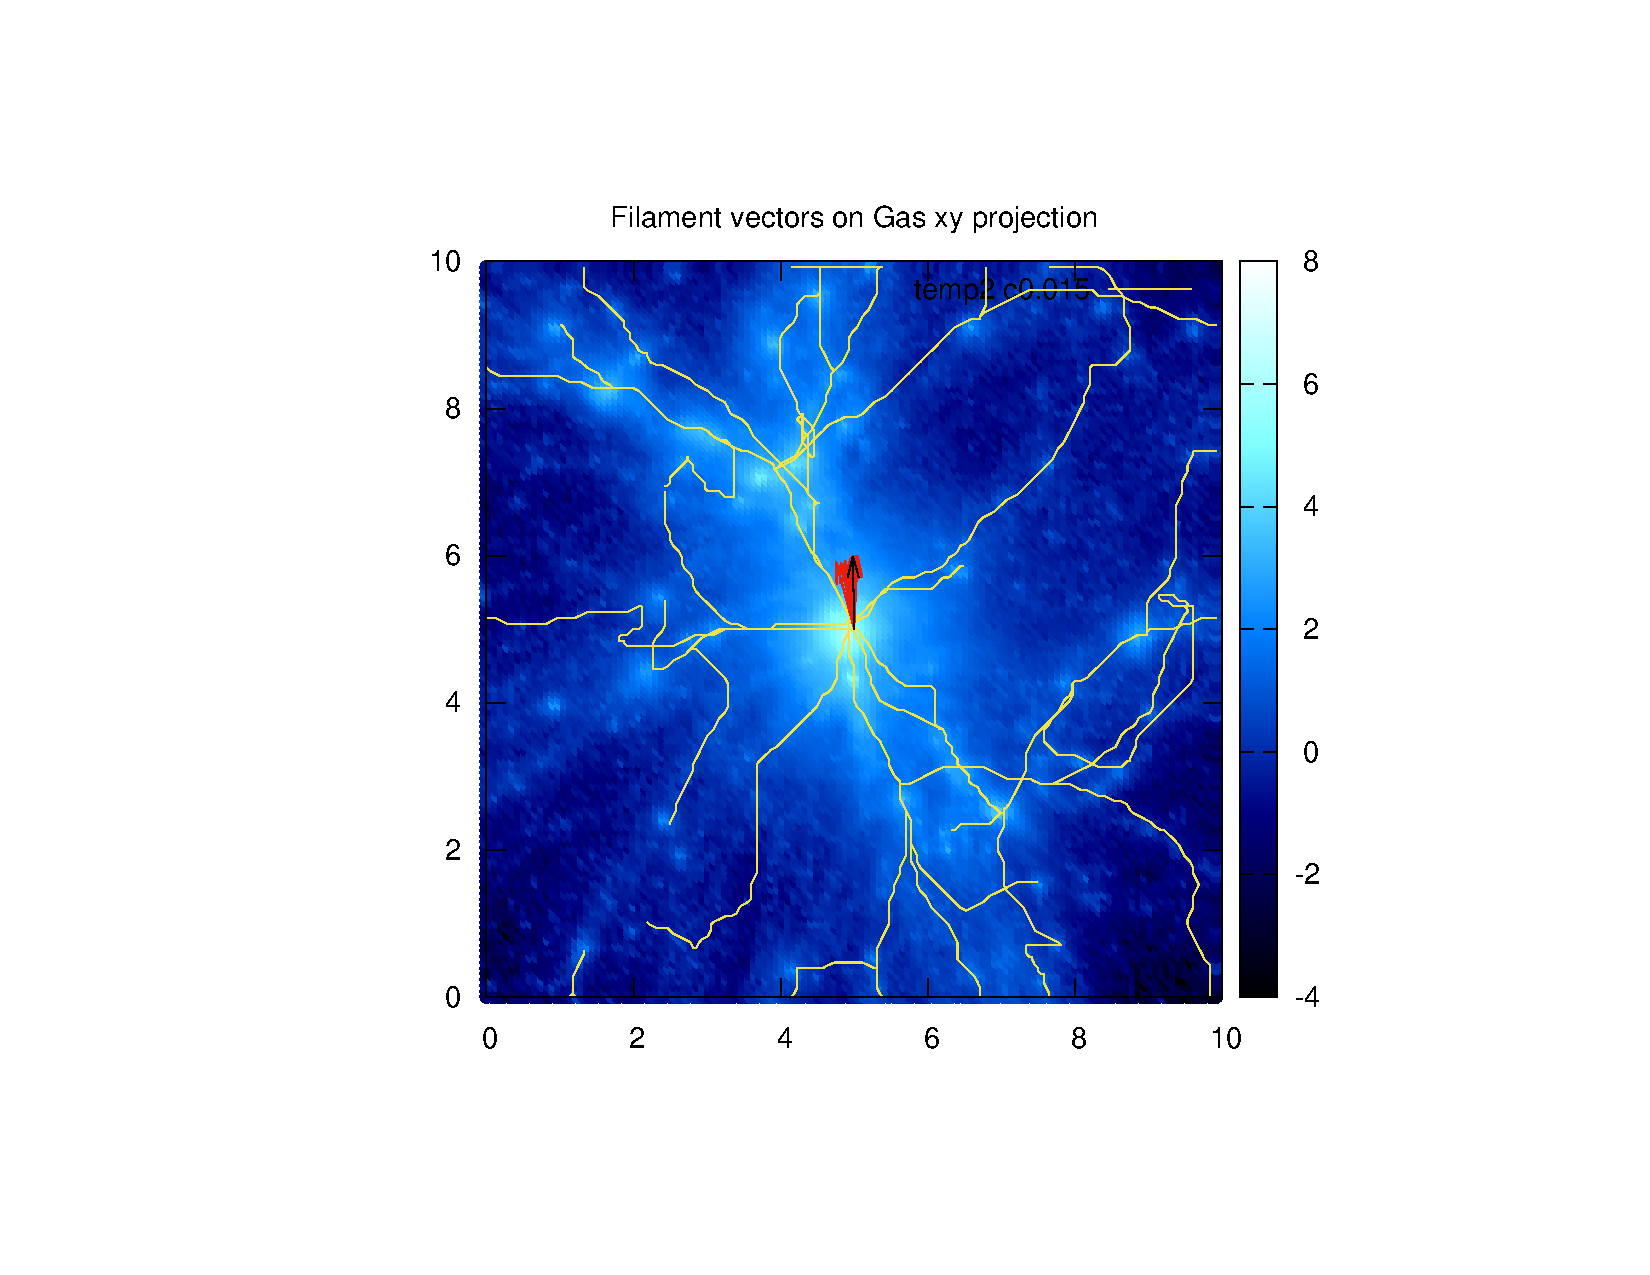
\includegraphics[width=\linewidth]{FilxyGas}
	\end{subfigure}
	\quad
	\begin{subfigure}[t]{0.3\textwidth}
		\centering
		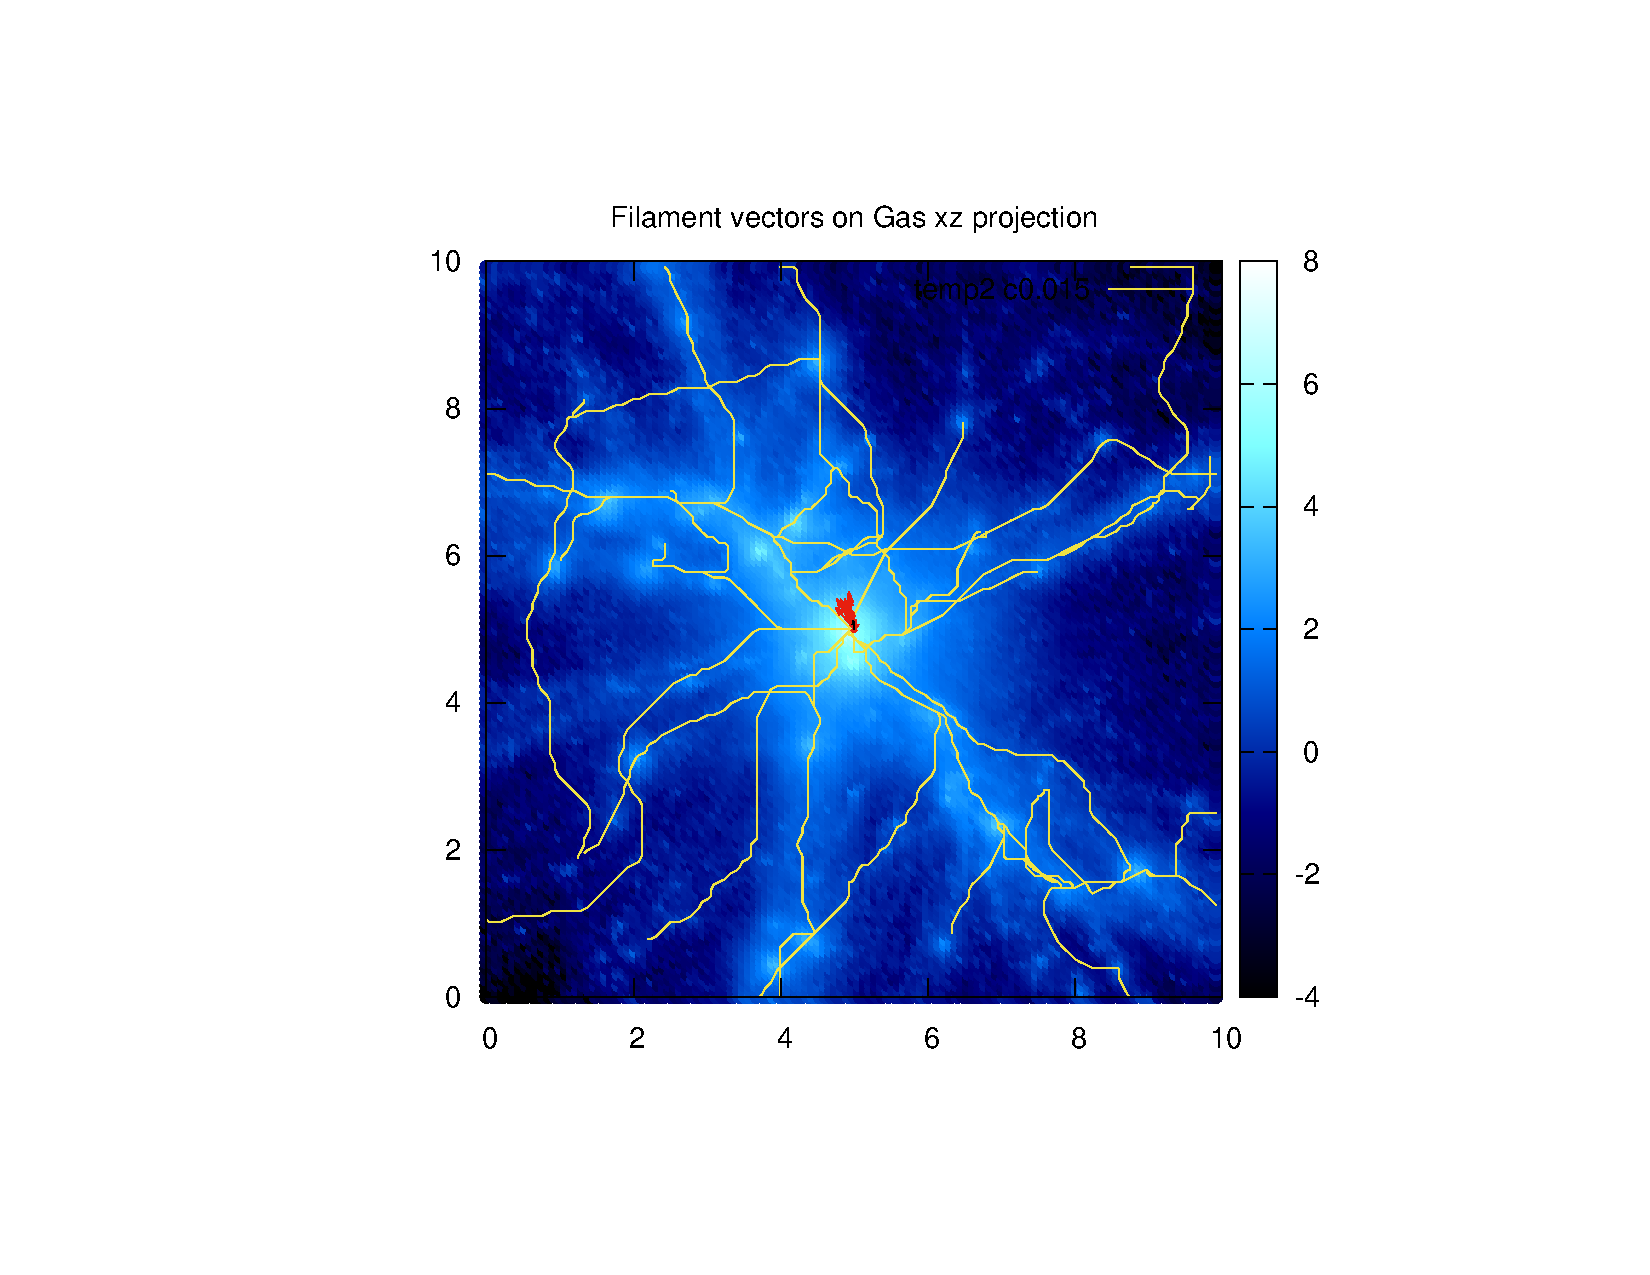
\includegraphics[width=\linewidth]{FilxzGas}
	\end{subfigure}
	\quad
	\begin{subfigure}[t]{0.3\textwidth}
		\centering
		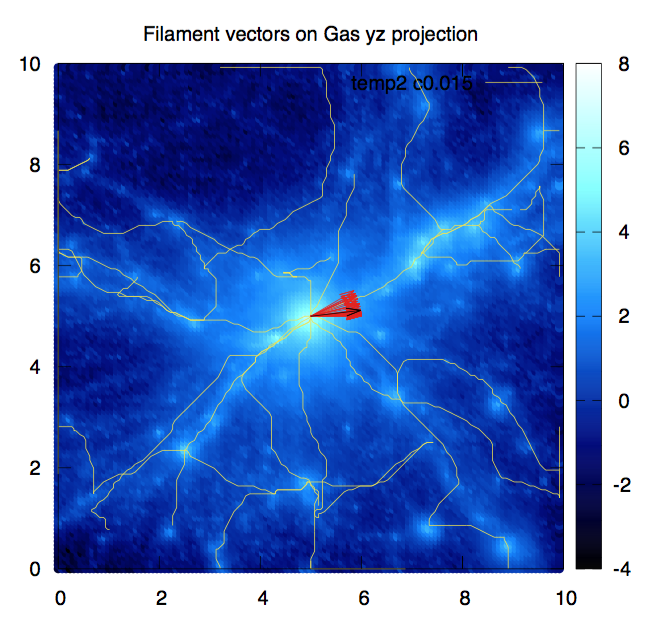
\includegraphics[width=\linewidth]{FilyzGas}
	\end{subfigure}
\label{fig:fil_calc}
	\caption{Filament vectors calculated for radii in range 1-5Mpc displayed on DM and Gas density background (red arrows) projections a) xy, b) xz and c) yz, with the averaged filament direction over all radii displayed in black.}
\end{figure*}

\subsection{Using DisPerSe to calculate filamentary structure}
The program DisPerSe \cite{sousbie11a}, standing for 'Discrete Persistent Structures Extractor' was developed by Sousbie et.al. to study the properties of filamentary structures in the cosmic web of galaxy distributions, by using the concept of persistence. The main idea is to find persistent topological structures within a data set, which can be of the form of an N-body particle set or a grid with values. These structures are identified as components of Morse-Smale complex of some input function defined over a manifold - this complex captures the relationship between the functions' gradient, its topology, and the topology of the manifold it is defined over. Further detail on this process is given in the Appendix.
The program DisPerSe outputs the skeleton structure for the given data set, which are plotted against the density background in Figure \ref{fig:densities}. From this skeleton structure, the unit directional vector of the corresponding filament is calculated within differing radii from the centre of mass. Each radii contains all segments from the overall skeleton that have extremities within the given sphere, as in Figure \ref{fig:fil_calc} a). From here the overall direction of the filament as defined from the centre of mass is calculated by averaging the separate segments, as in Figure \ref{fig:fil_calc}. Due to the small number of segments included in any radius smaller than 1 Mpc away from the centre of mass, these filament direction was only calculated for a radius range of 1-5 Mpc. From this set of filament unit vectors, a single averaged filament direction was calculated (shown in black on Figure \ref{fig:fil_calc}) and used as a constant in further calculations.
\subsection{Pawsey Resources}
The Horizon-AGN data set is located on the Pawsey Supercomputer Magnus in the scratch directory, and is currently being worked on by a PhD student looking to develop a halo-finder algorithm, which would allow these results to be extended to the much larger dataset. The nIFTy cluster is a much smaller dataset, and so this analysis was capable of being conducted on a personal computer. Use was made of the NECTAR resource to run the DisPerSe program, as a higher amount of memory was required to compute the Morse-Smale complex. Although no jobs were run on Magnus throughout this project, the idea was to formulate an automated process that could be applied to a large data set of many halos, which would be easily applicable to the Horizon-AGN data set. 


\begin{figure*}[!t]
\centering
	\begin{subfigure}[t]{0.45\textwidth}
		\centering
		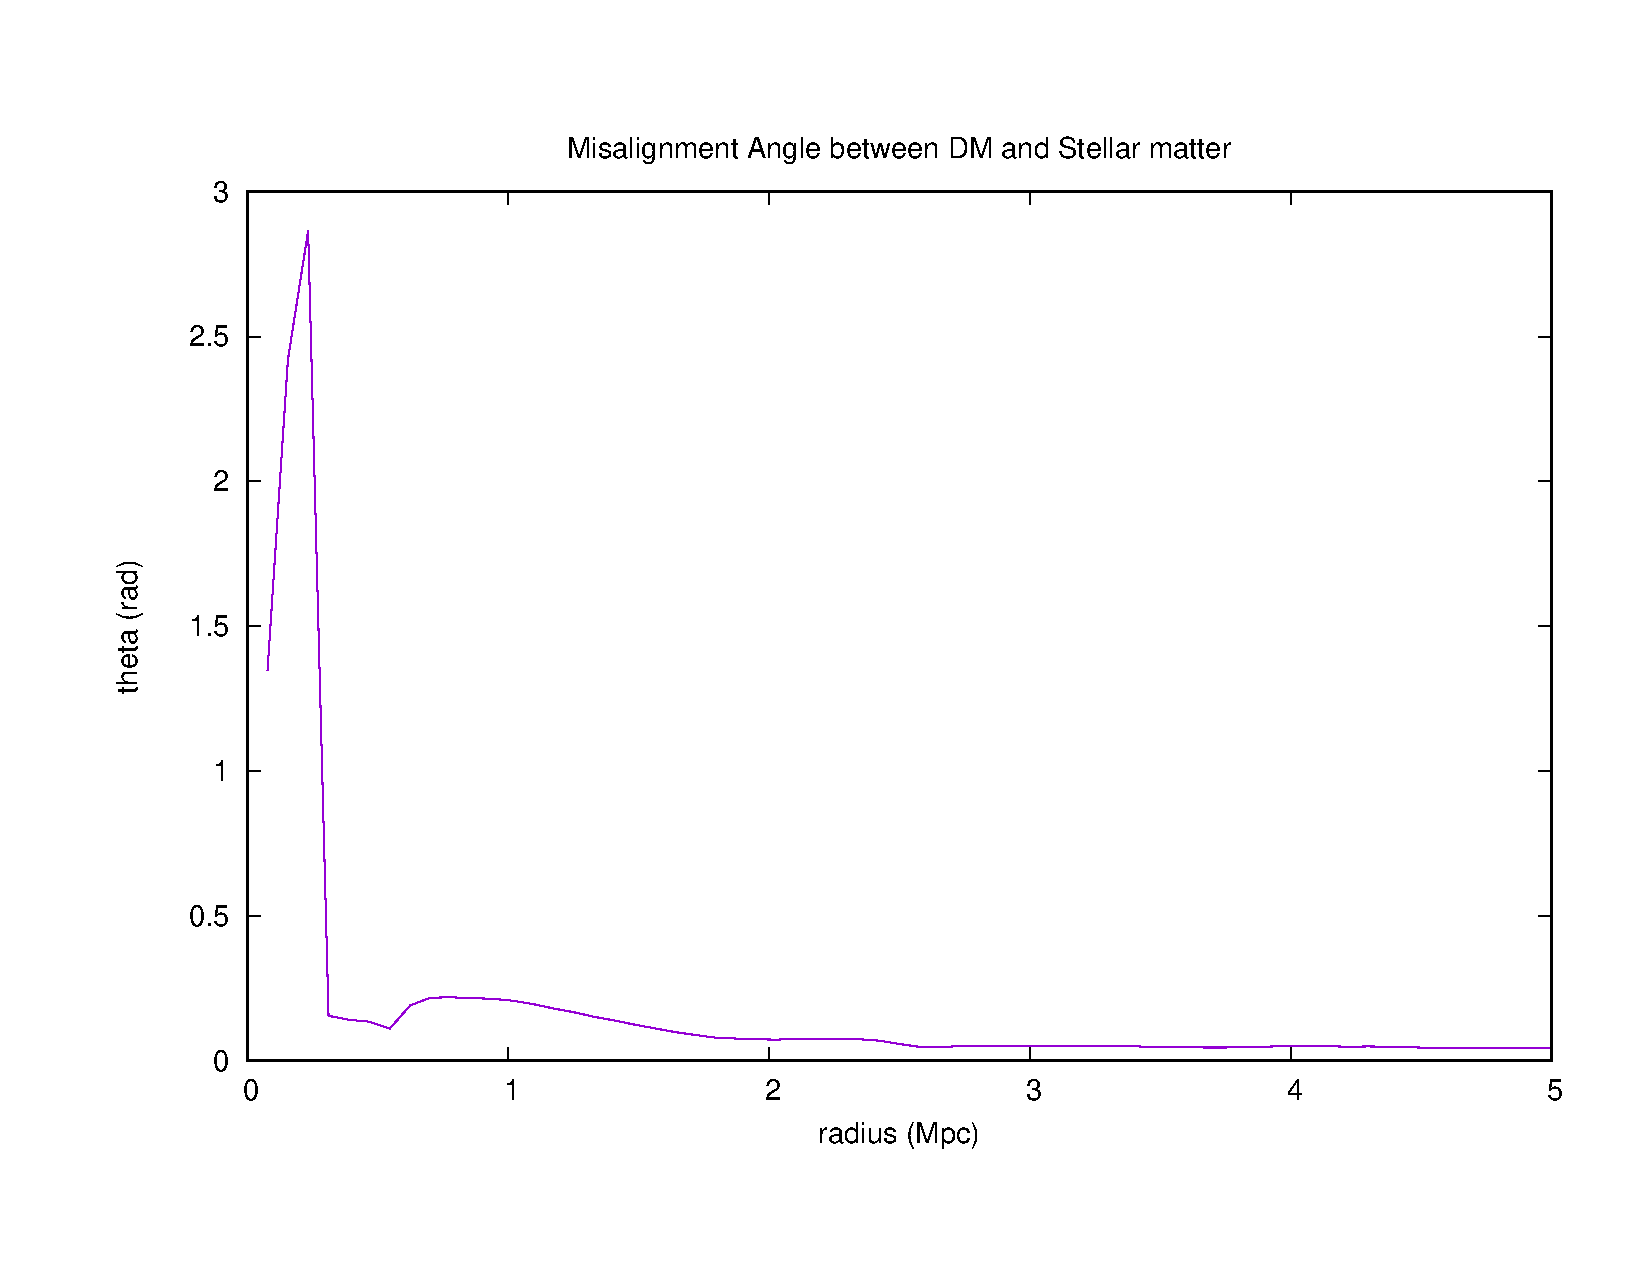
\includegraphics[width=\linewidth]{GasDMAlign}
	\end{subfigure}
	\quad
	\begin{subfigure}[t]{0.45\textwidth}
		\centering
		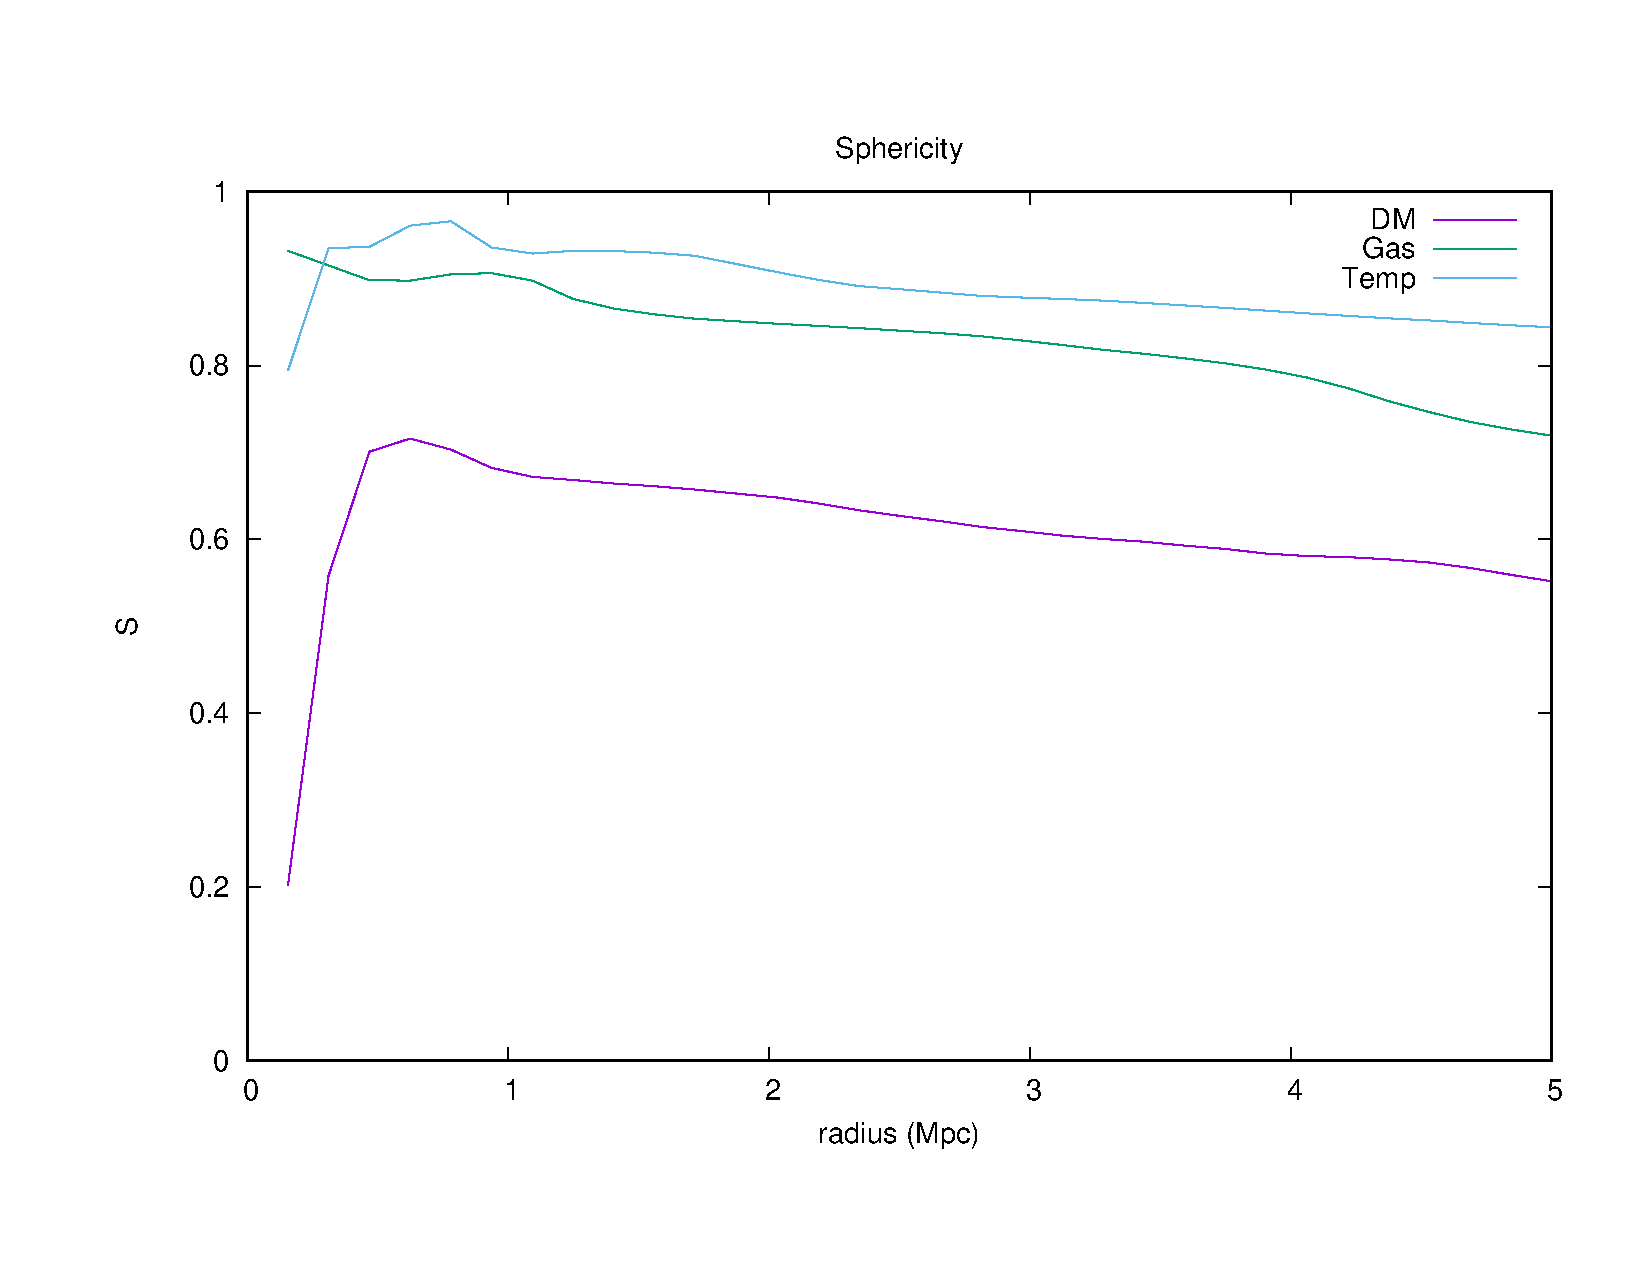
\includegraphics[width=\linewidth]{Sphericity}
	\end{subfigure}
	\\
	\begin{subfigure}[t]{0.45\textwidth}
		\centering
		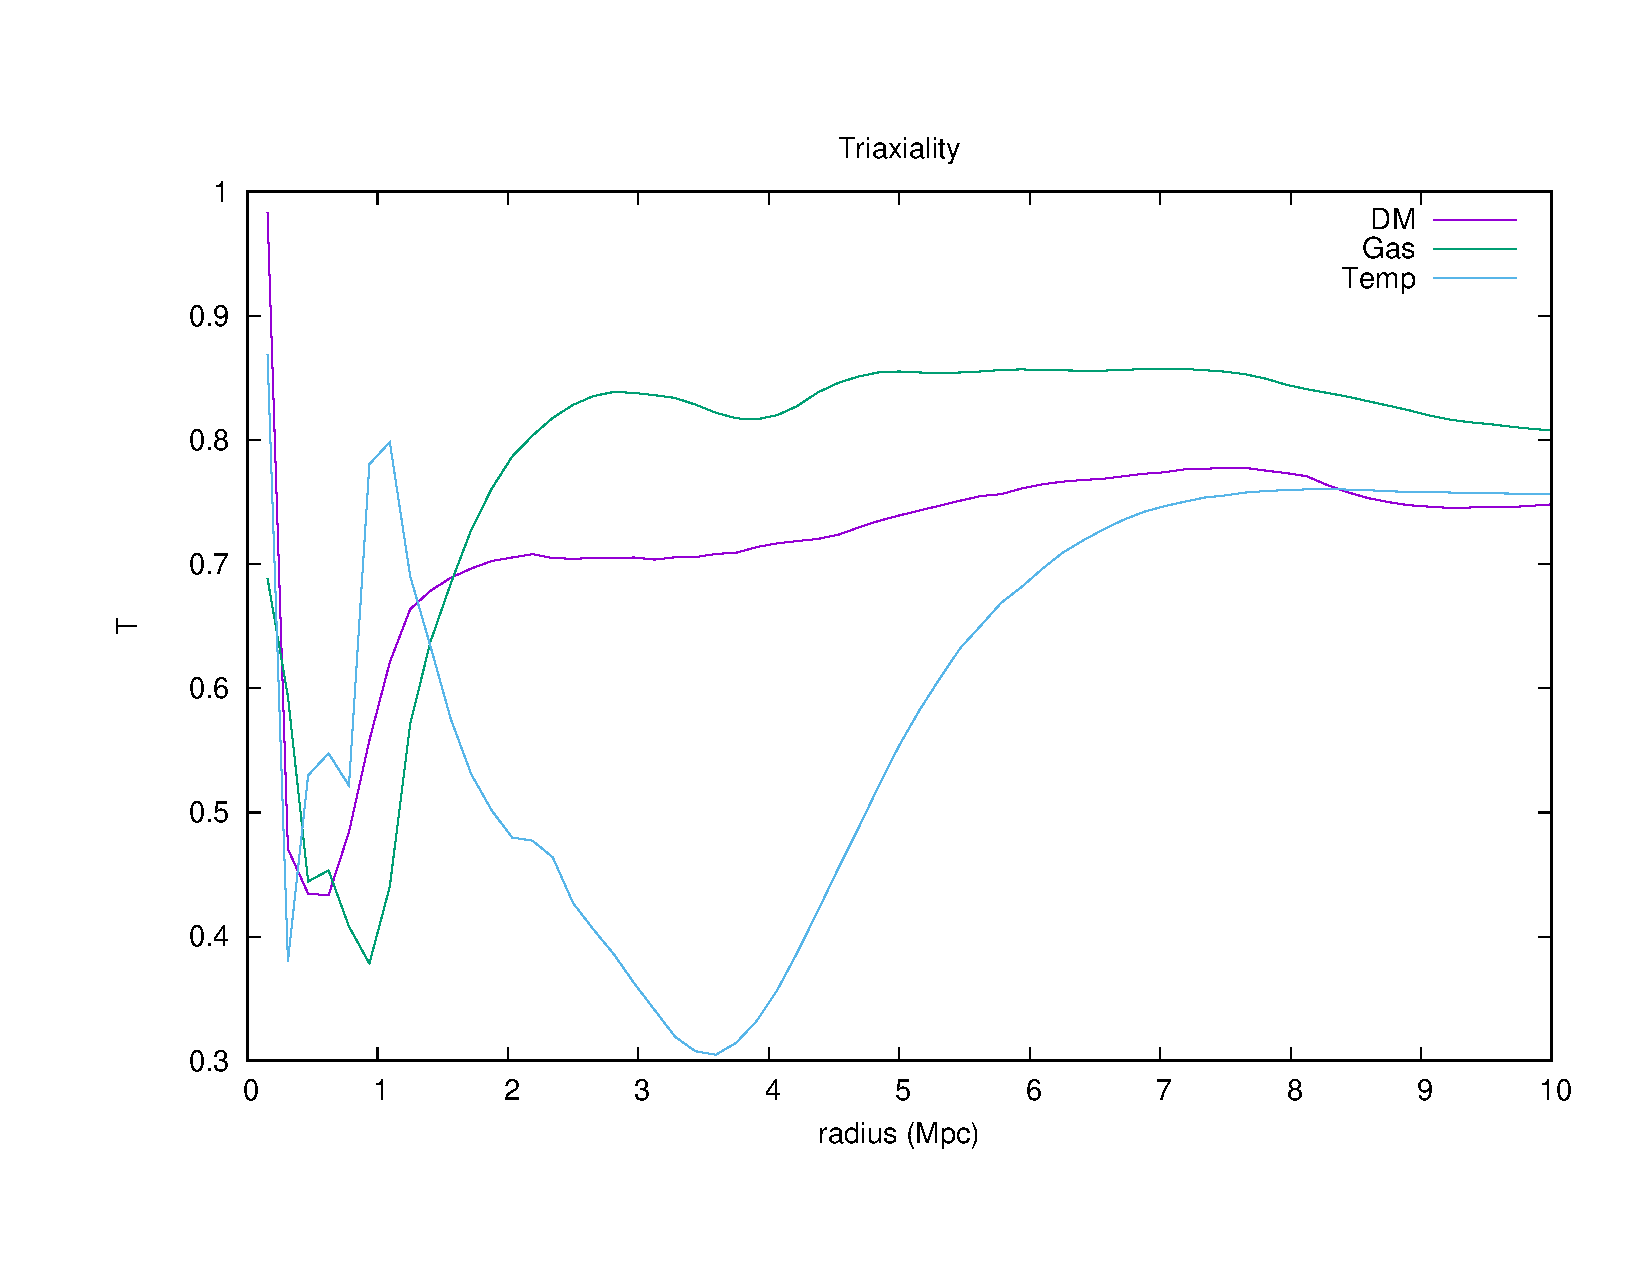
\includegraphics[width=\linewidth]{Triaxiality}
	\end{subfigure}
	\quad
	\begin{subfigure}[t]{0.45\textwidth}
		\centering
		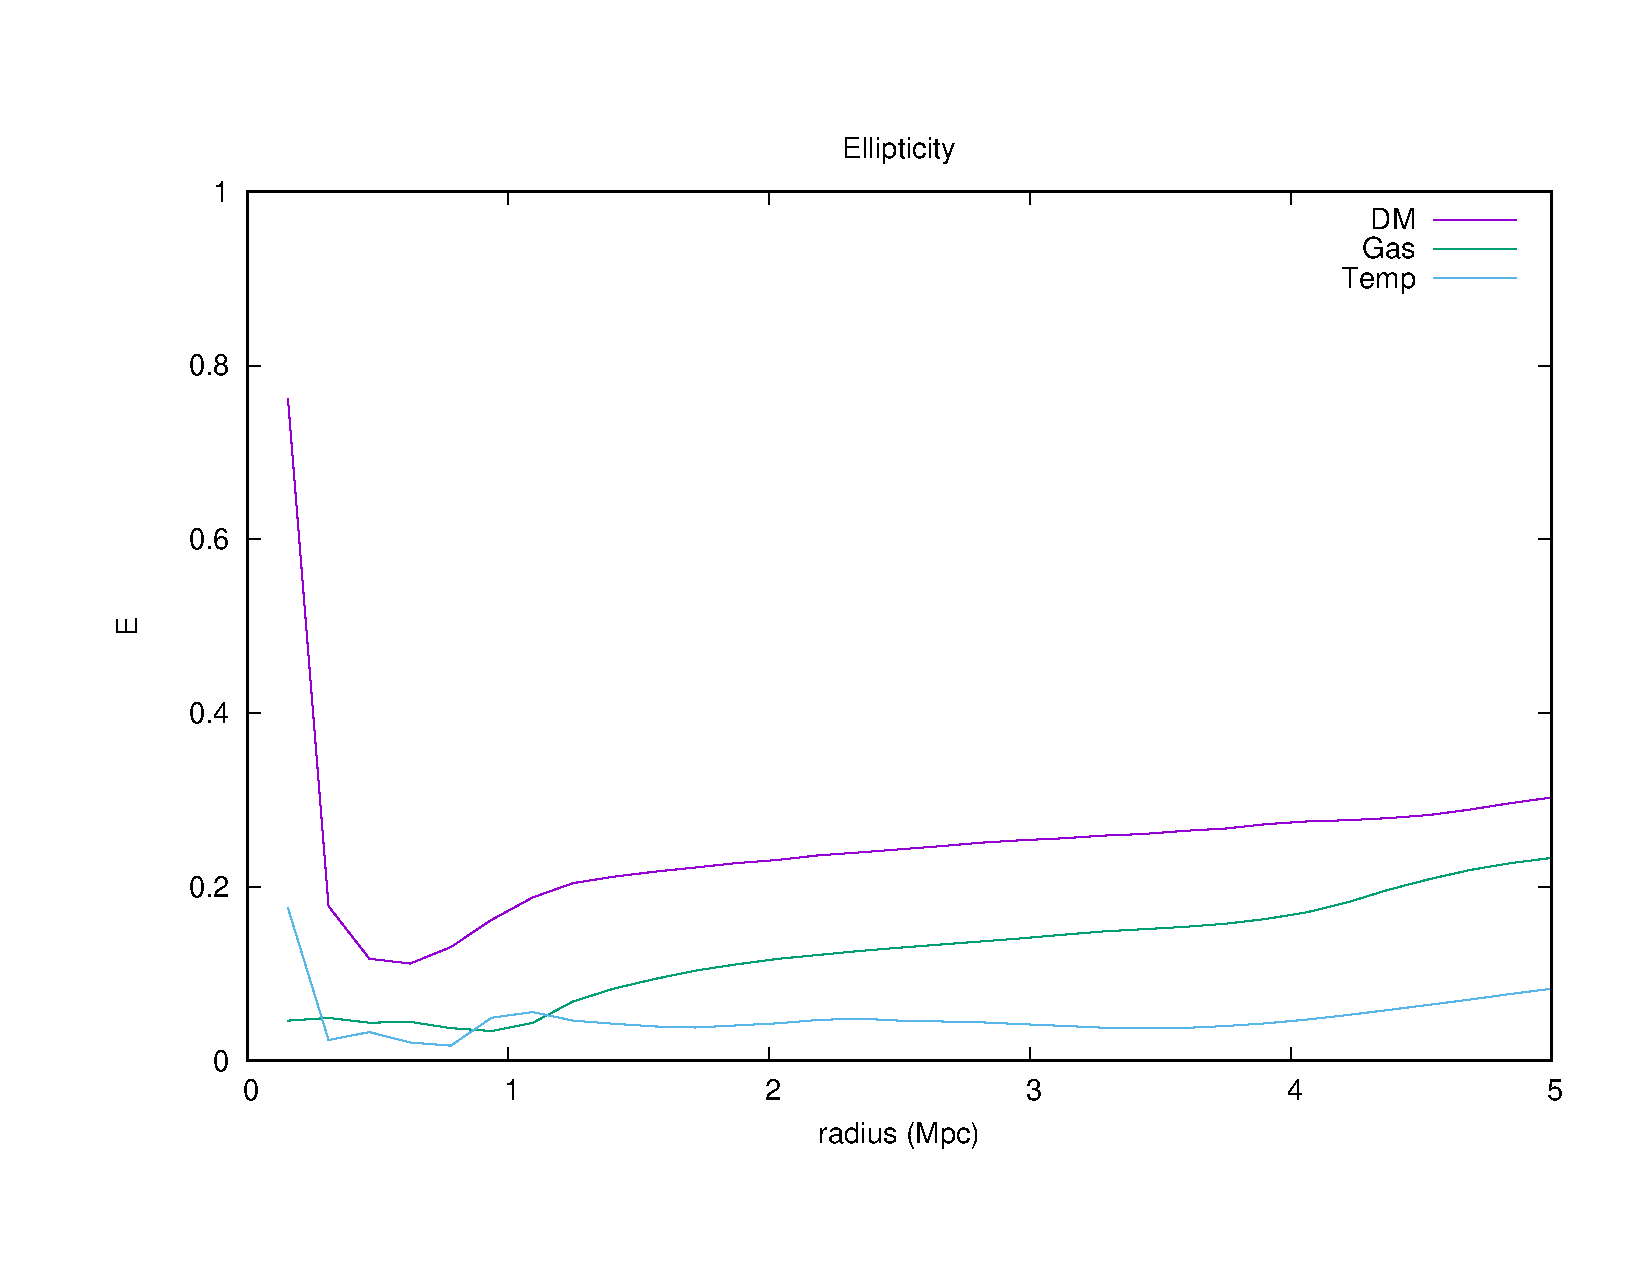
\includegraphics[width=\linewidth]{Ellipticity}
	\end{subfigure}
\caption{Misalignment angle between DM and stellar matter in a) and shape properties of DM, stellar matter and temperature for the halo using b) sphericity, c) triaxiality and d) ellipticity.}
\label{fig:shapes}
\end{figure*}


\section{Results}
\subsection{Ellipsoid plots on density background}
\textit{What features are observed? How do these plots vary at different radii - do they show a higher level of alignment? More sphericity? 
Misalignment angle between stellar and DM components}
As expected, the plots of ellipsoid using the major axes from the eigenvalues of the moment of inertia tensor show significant elongation along the filament direction in all 2D projections, as is expected in the hierarchical model whereby clusters form as matter infalls along the filament. The DM plots show more elliptical shapes than the stellar matter, and the temperature plots maintain a roughly spherical profile throughout. It can be seen that closer to the centre of mass the ellipses become spherical in shape, corresponding to a higher density yet more consistent spread within the smaller radii. 
The high level of sphericity (and hence confusion in calculation of the major axis direction) corresponds also to high level of misalignment between the major axes of DM and stellar components as seen in Figure \ref{fig:shapes} a). 

\subsection{Sphericity, Triaxiality and Ellipticity of different matter}
\textit{What defining features are seen in plots of sphericity and ellipticity against radius? What are the differences between stellar and DM? How does the temperature plot give any further information?
(Introduce the idea of a confounding merger and show in pictures)}

The plots of sphericity in Figure \ref{fig:shapes} show that overall the DM in the cube has a lower overall sphericity, with both stellar matter (gas) and temperature profiles showing a higher sphericity. The sphericity for the temperature profile peaks at a radius of approximately 0.8 Mpc out from the halo centre of mass, corresponding to a virial shock seen on the density plots. The stellar matter sphericity peaks slightly further out at a radius of about 1 Mpc, but still related to the temperature peak as would be expected. The higher radius for the Gas profile corresponds to the stellar material being blown out away from the centre of mass by the shock. 
The plot of triaxiality in Figure \ref{fig:shapes} shows significant inconsistency at lower radii, however at higher radii as matter tends to stream along the filament, it is clear that the stellar matter is more elongated along the poles (assumed to be along the filament inflow) whereas the DM is slightly less elongated. The temperature retains a much more spherical profile.
The plot of ellipticity in Figure \ref{fig:shapes} shows that the DM has a higher ellipticty than both stellar matter and the temperature profile. It can be seen that at a radius of about 1 Mpc the temperature briefly has a more elliptic profile than the stellar matter, which corresponds to where the sphericity peaked (which makes sense physically), and can be connected to the virial shock seen on density plots (reference figure that has gas density plotted with circle at centre of mass of radius 1 Mpc). Unlike the temperature profile, the stellar matter increases its ellipticity until it is almost on par with that of the DM at radius of 5 Mpc (at the edge of the simulation cube), likely due to the fact that 

It is interesting to note the difference between the major axes of the DM and stellar matter, as plotted in Figure \ref{fig:DMgasAlign}. The spike in misalignment at a low radius is likely due to the high sphericity of both matters at very small radii from the centre of mass (as discussed above) which confounds the measurement of an accurate major axis. However there is a noticeable peak at a radius of 1 Mpc out from the centre of mass, the same point at which the temperature profile has higher ellipticity than the gas, i.e. the point at which the gas has an increase in sphericity, corresponding to the blow out of stellar material in a virial shock.

\subsection{Skeleton plots and filament construction at small radii}
\textit{How does the filament angle change when calculated at smaller radii around the centre of mass?
How does the alignment of the stellar/DM components with the filament change for different radii?
Which is generally more aligned with the filament, the stellar or DM component?}

\begin{figure*}[!t]
\centering
	\begin{subfigure}[t]{0.45\textwidth}
		\centering
		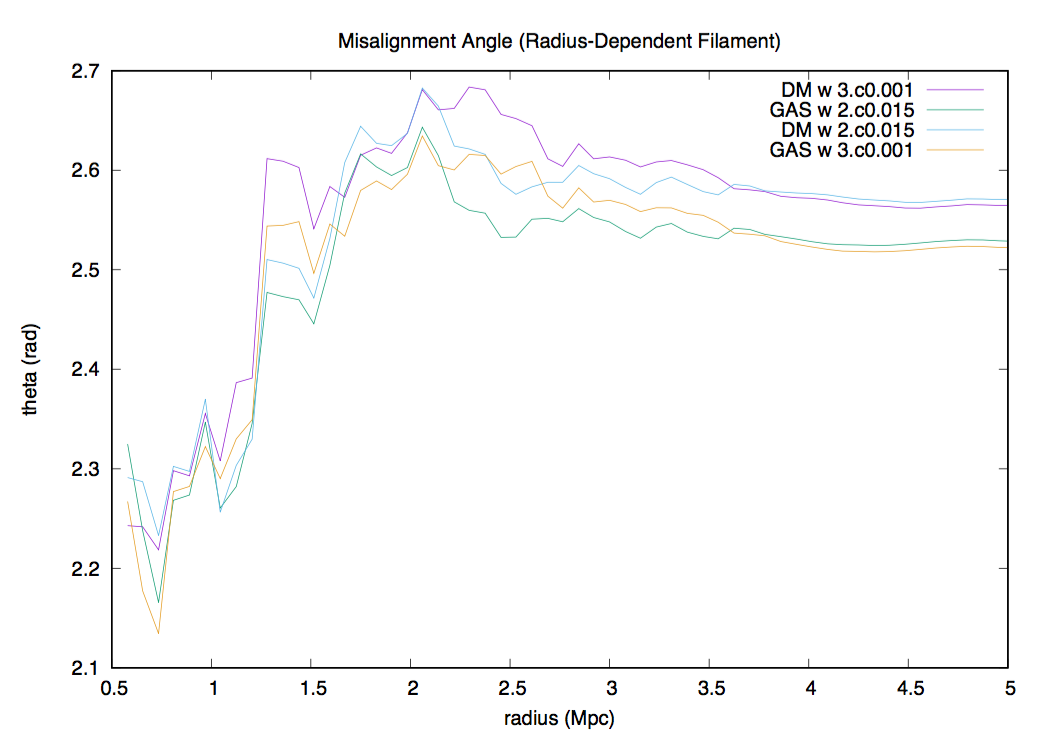
\includegraphics[width=\linewidth]{MisRad}
	\end{subfigure}
	\quad
	\begin{subfigure}[t]{0.45\textwidth}
		\centering
		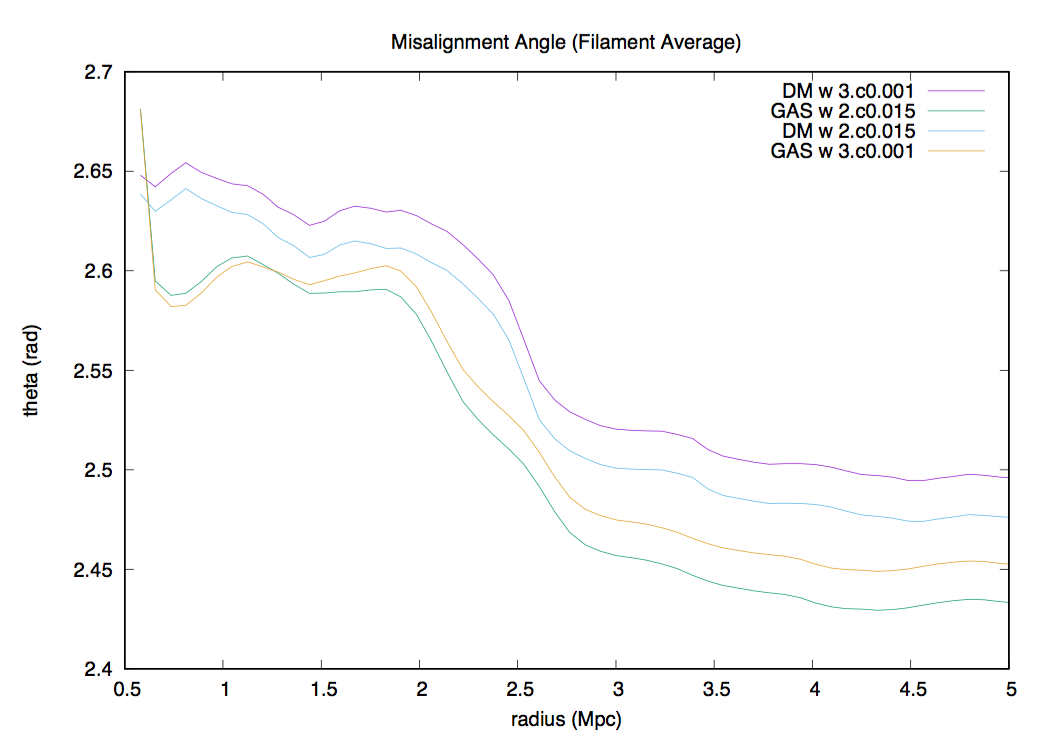
\includegraphics[width=\linewidth]{MisAve}
	\end{subfigure}
\label{fig:angleplots}
	\caption{Plots of the angle between the filament direction and the major axis for the halo calculated using the reduced moment of inertia tensor at different radii from the centre of mass for a) radius-dependent filament directions and b) the averaged filament direction over all radius.}
\end{figure*}

%%%% TEMPERATURE PLOTS ON GAS SKELETON %%%%
\begin{figure*}[!t]
%\centering
	\begin{subfigure}[t]{0.3\textwidth}
		\centering
		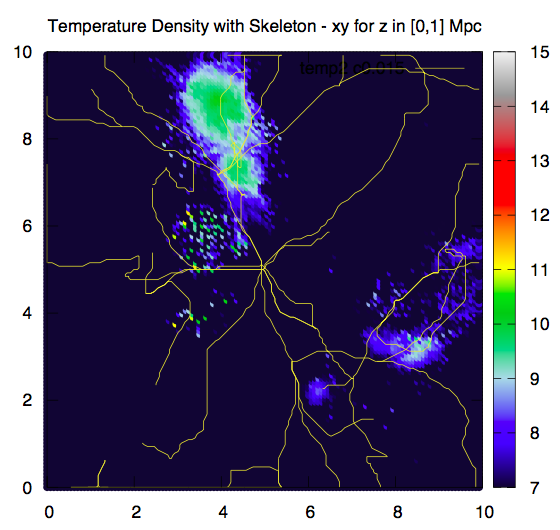
\includegraphics[width=\linewidth]{TempDenSkel01}
	\end{subfigure}
	\quad
	\begin{subfigure}[t]{0.3\textwidth}
		\centering
		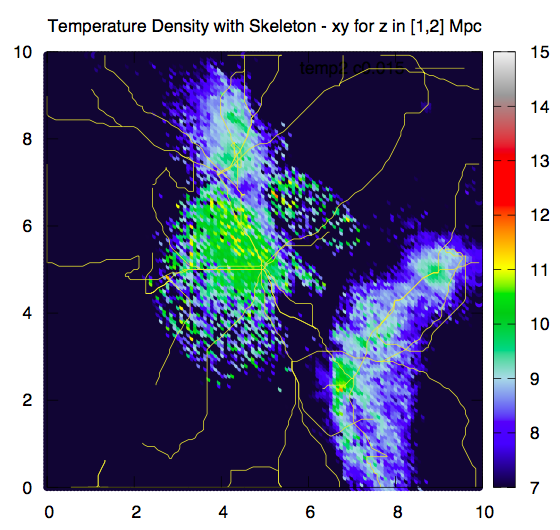
\includegraphics[width=\linewidth]{TempDenSkel02}
	\end{subfigure}
	\quad
	\begin{subfigure}[t]{0.3\textwidth}
		\centering
		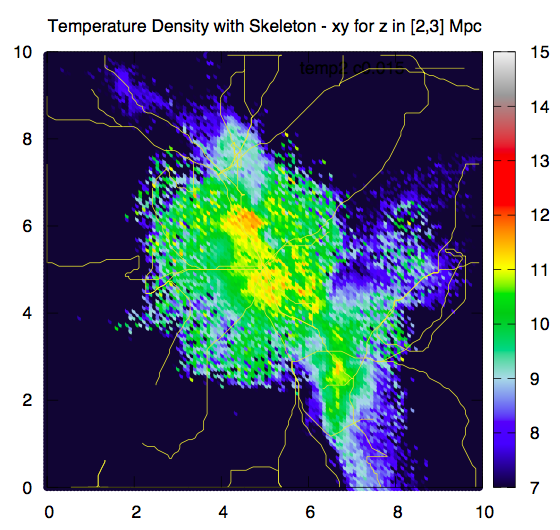
\includegraphics[width=\linewidth]{TempDenSkel03}
	\end{subfigure}
	\\
	\begin{subfigure}[t]{0.3\textwidth}
		\centering
		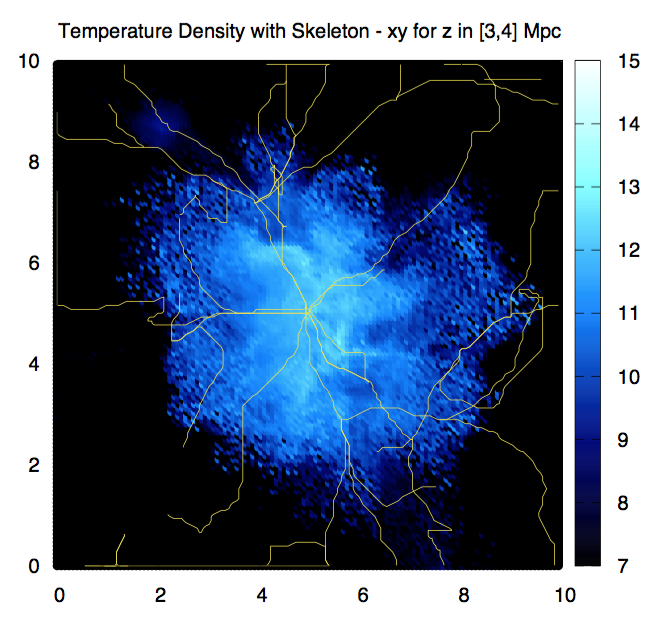
\includegraphics[width=\linewidth]{TempDenSkel04}
	\end{subfigure}
	\quad
	\begin{subfigure}[t]{0.3\textwidth}
		\centering
		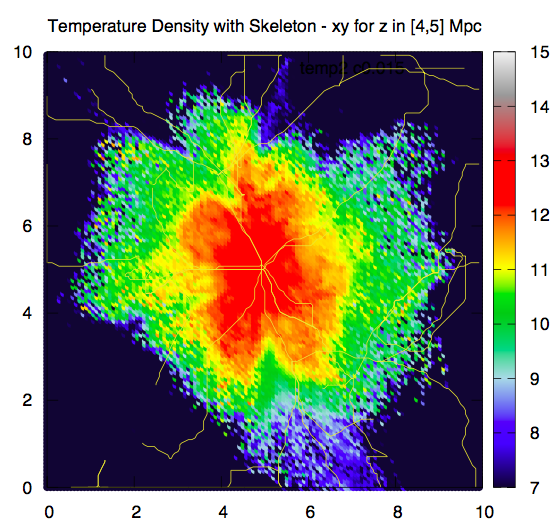
\includegraphics[width=\linewidth]{TempDenSkel05}
	\end{subfigure}
	\quad
	\begin{subfigure}[t]{0.3\textwidth}
		\centering
		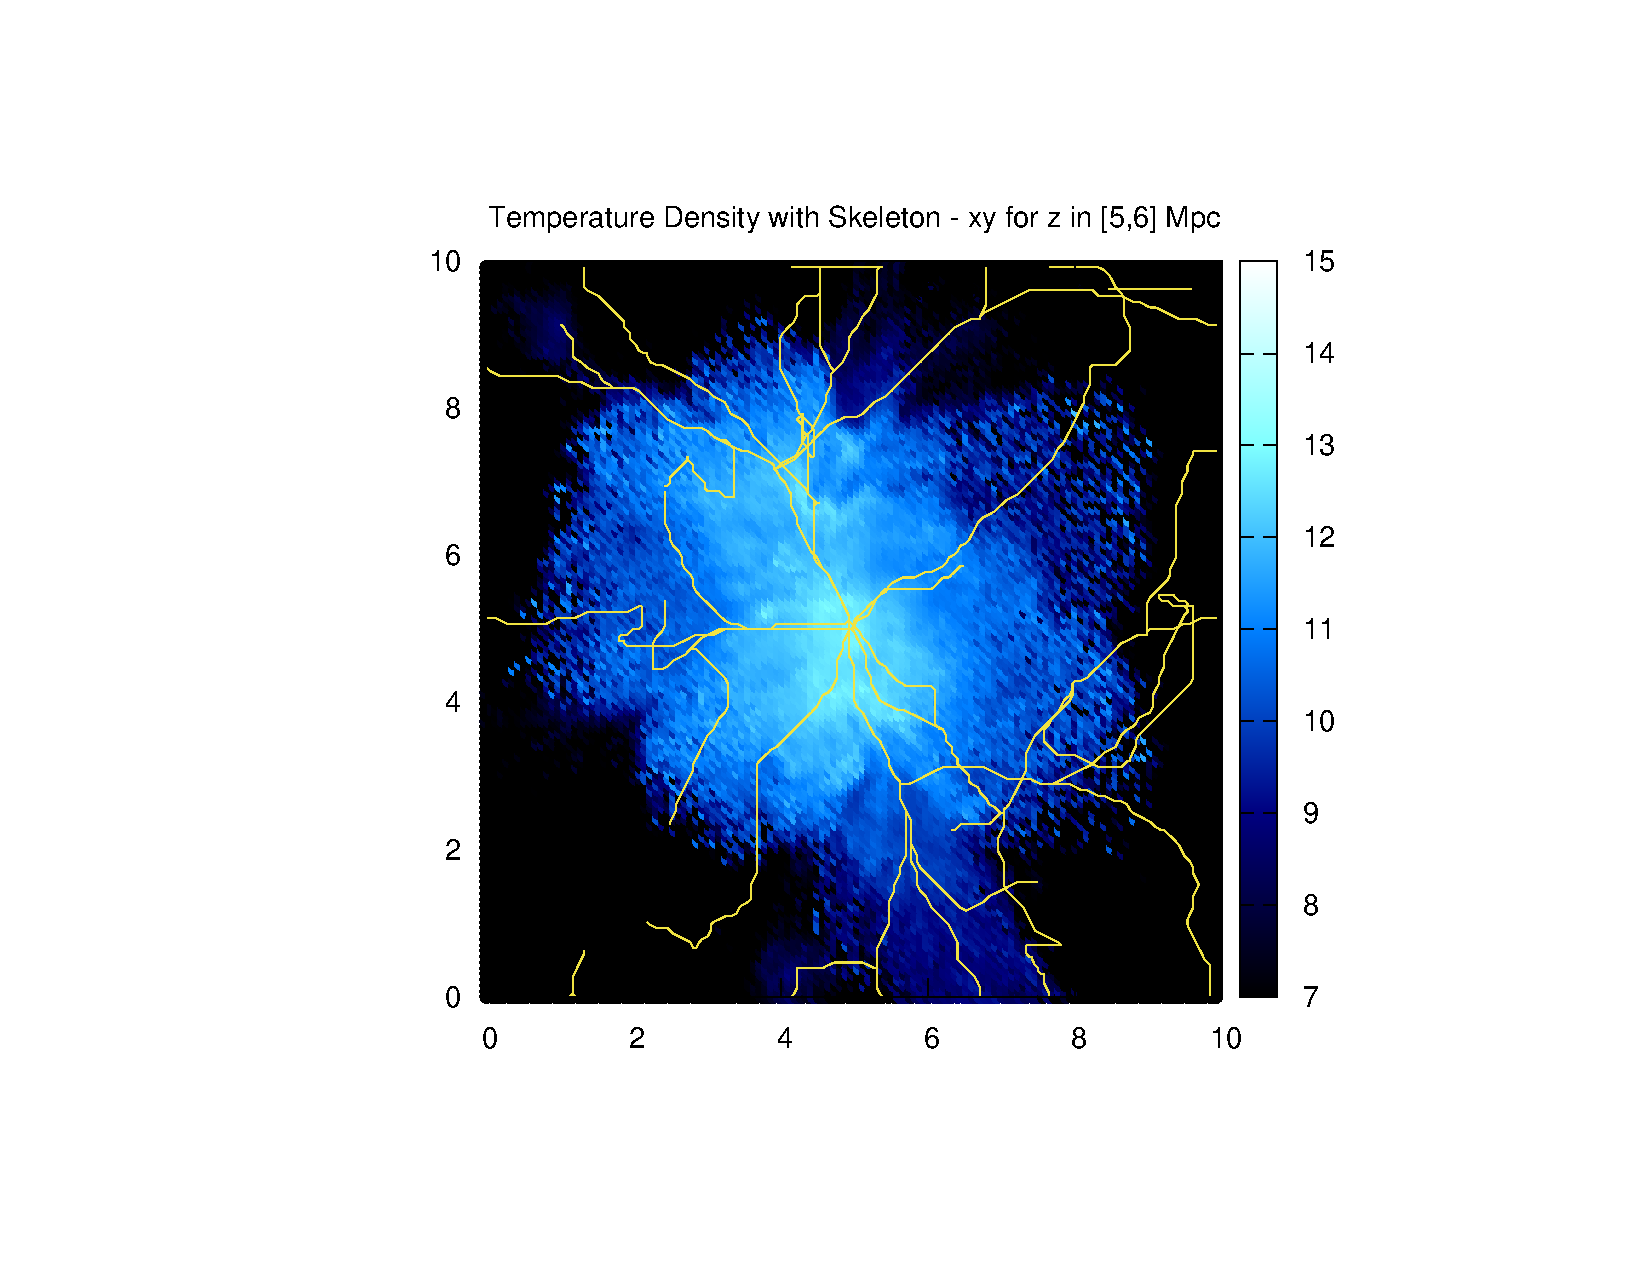
\includegraphics[width=\linewidth]{TempDenSkel06}
	\end{subfigure}
	\\
	\begin{subfigure}[t]{0.3\textwidth}
		\centering
		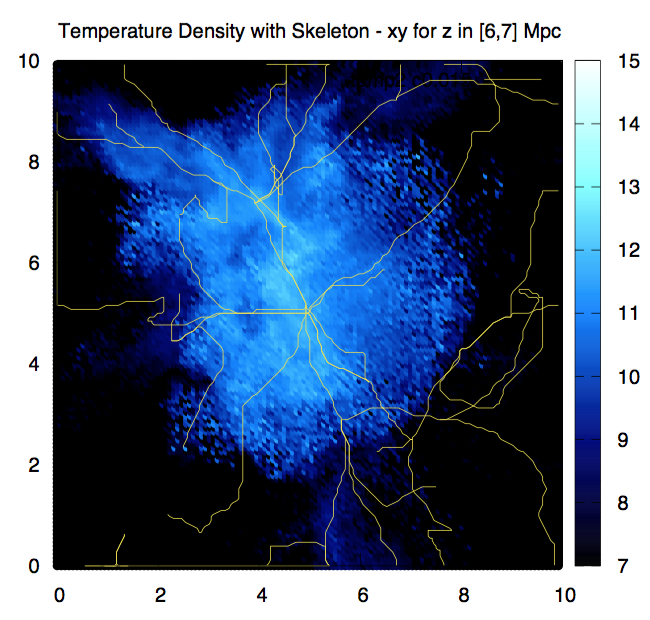
\includegraphics[width=\linewidth]{TempDenSkel07}
	\end{subfigure}
	\quad
	\begin{subfigure}[t]{0.3\textwidth}
		\centering
		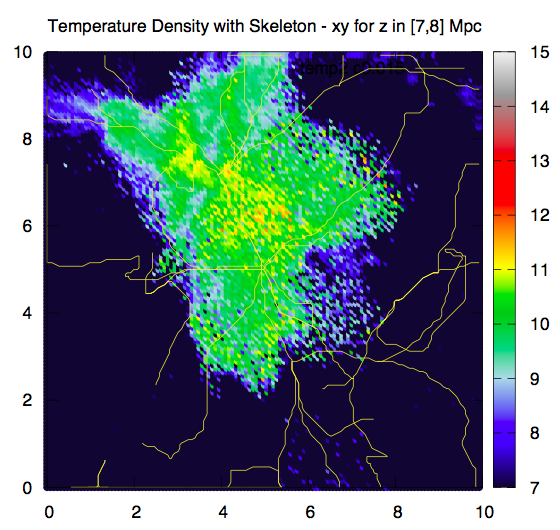
\includegraphics[width=\linewidth]{TempDenSkel08}
	\end{subfigure}
	\quad
	\begin{subfigure}[t]{0.3\textwidth}
		\centering
		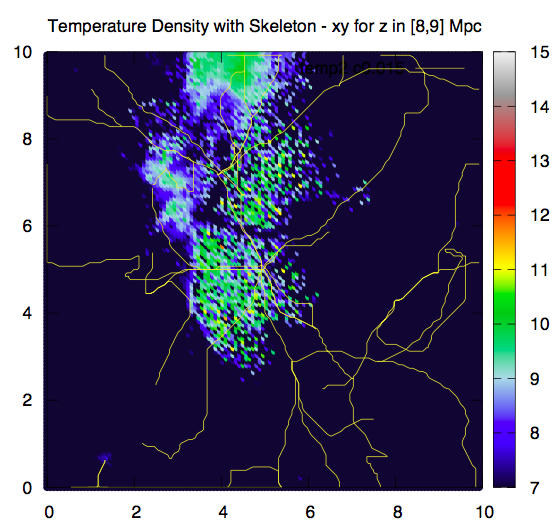
\includegraphics[width=\linewidth]{TempDenSkel09}
	\end{subfigure}
	\\
	\begin{subfigure}[t]{0.3\textwidth}
		\centering
		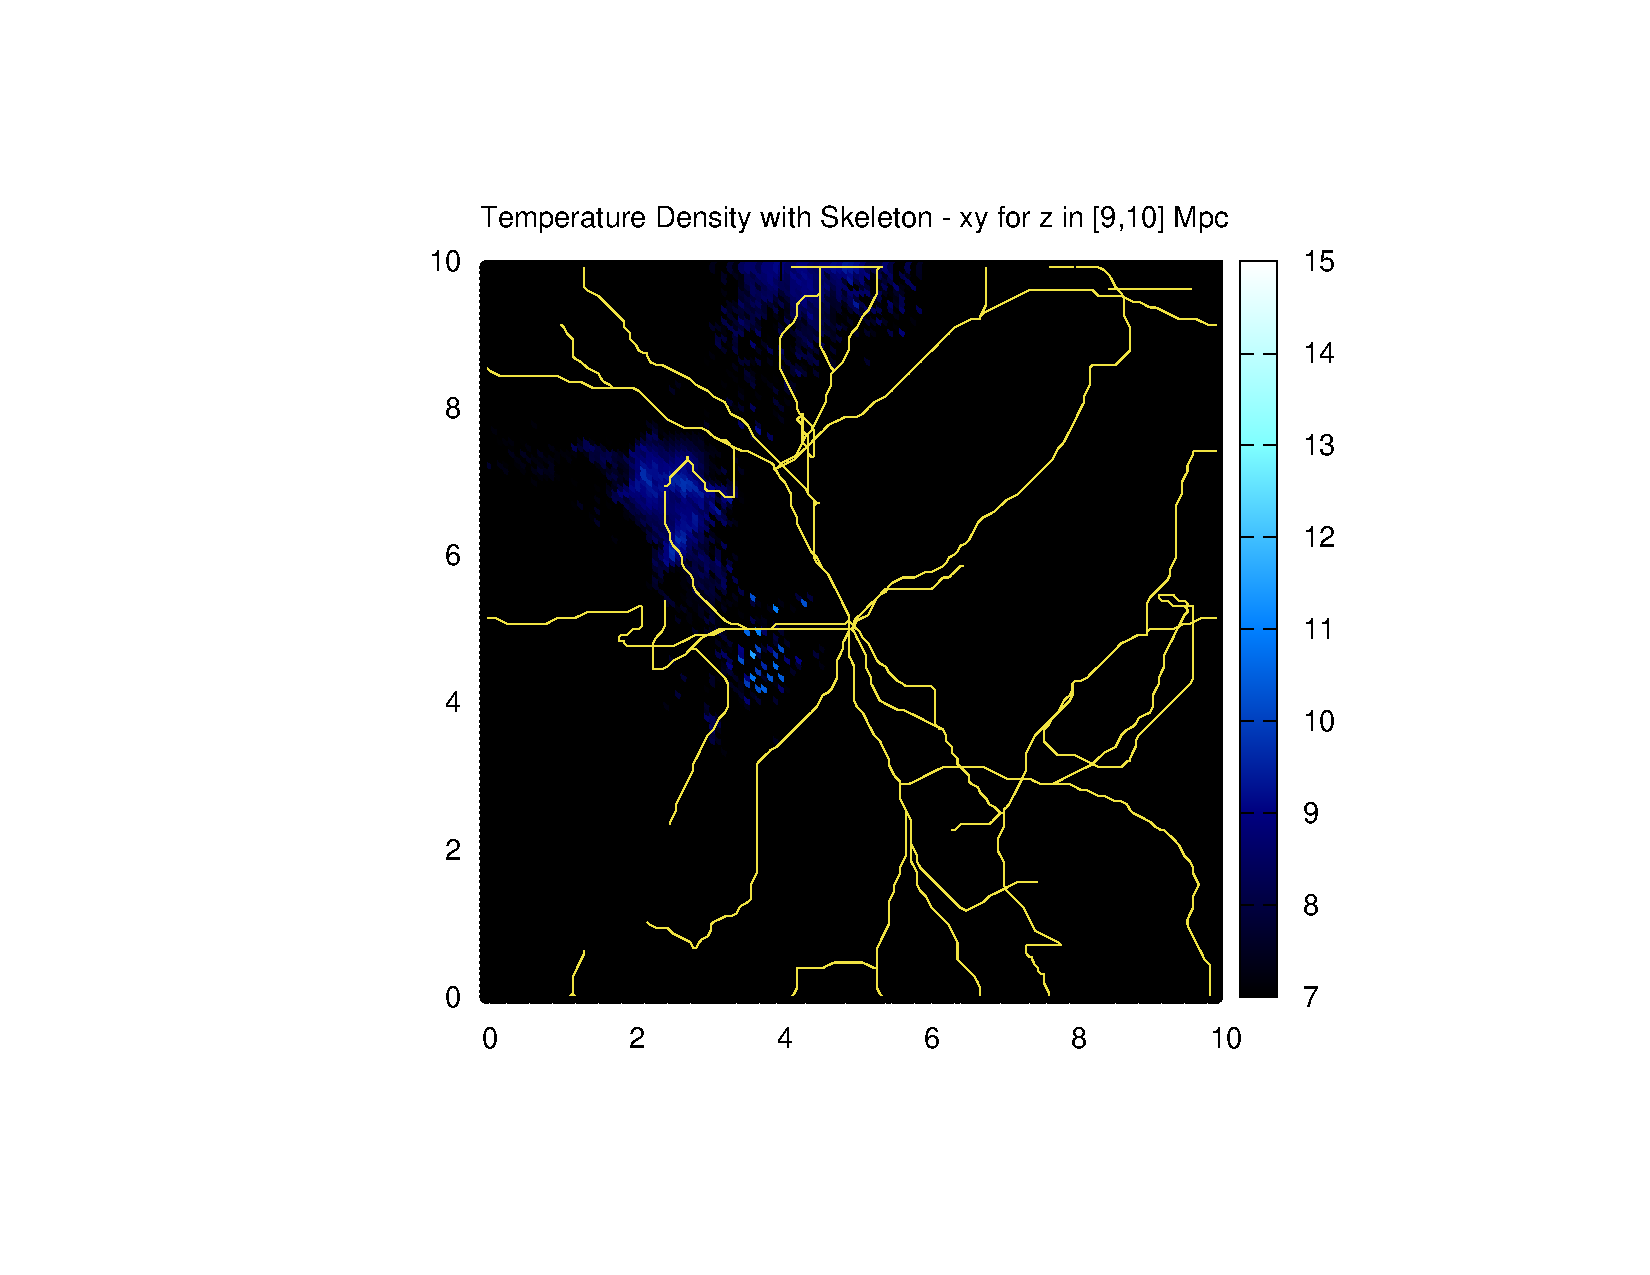
\includegraphics[width=\linewidth]{TempDenSkel10}
	\end{subfigure}
	\quad
	\begin{subfigure}[t]{0.3\textwidth}
		\centering
		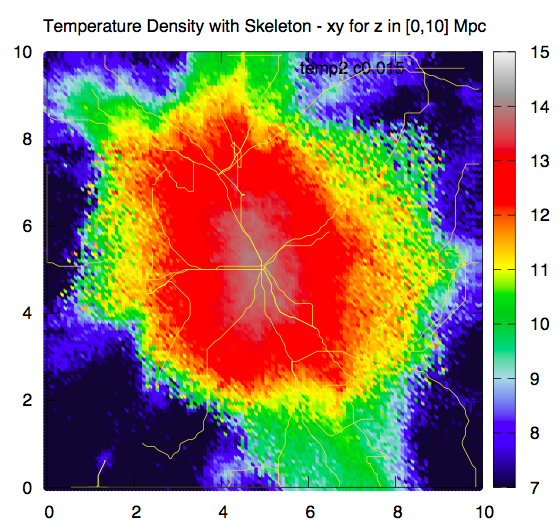
\includegraphics[width=\linewidth]{TempDenSkelall}
	\end{subfigure}
\label{fig:tempskel}
\caption{Sliced temperature density profiles in xy projection with overlaid Gas skeleton.}
\end{figure*}

\section{Conclusion}
\textit{Very brief - one paragraph on what was interesting, what could be investigated, how the study could be moved up to a large data set (e.g. what was the most important statistic - the alignment of stellar halo with filament).
What does this have to say about hierarchical structure formation? How much of a confounding effect can we expect major mergers to have on any large data set that this process was conducted on?}


%%%%% APPENDIX %%%%%
\appendices
\section{The Morse-Smale Complex and Persistence}
Critical points are discrete sets of points where the Morse function's gradient is null, and integral lines are curves tangent to the gradient field at every point. Integral lines cover all space and their extremities are critical points, which induces a tesselation of space into regions called ascending manifolds. The set of these ascending manifolds is the Morse complex of the function. The Morse-Smale complex is an extension of this concept - the space is tesselated into regions called 'p-cells', each of which is the intersection of an ascending and descending manifold. 
Topological components of a function can be represented by pairs of positive and negative critical points called persistence pairs - where a positive critical point corresponds to a created topological component, and a negative to a destroyed topological component. The absolute difference between the value of the critical points in a pair is the persistence, which represents the lifetime of the corresponding component. DisPerSe allows the specification of a persistence threshold which allows removal of topological components with persistence lower, hence filtering noise from the Morse-Smale complex. 

\section*{Acknowledgment}
I would like to thank both my supervisors, Dr Chris Power and Dr Charlotte Welker, for their assistance on this project and for sharing their valuable time. Also the staff at ICRAR, who were extremely helpful and formed such an inclusive community. I would also like to thank Chris Bording, for all his assistance with working with the Pawsey Resources as well as much else. 

%%%%% REFERENCES %%%%%
\begin{thebibliography}{1}

\bibitem{white78}
	S.D.M.~White and M.J.~Rees, 1978, \emph{Core condensation in heavy halos: a two-stage theory for galaxy formation and clustering}, \hskip 1em MNRAS 183 p.341-358.
\bibitem{davis85}
	M.~Davis,G.~Efstathiou,C.S.~Frenk and S.D.M.~White, 1985, \emph{The evolution of large-scale structure in a universe dominated by cold dark matter}, \hskip 1em The Astrophysical Journal 292 p.371-394.
\bibitem{lemson99}
	G.~Lemson and G.~Kauffmann, 1999, \emph{Environmental influences on dark matter haloes and consequences for the galaxies within them},\hskip 1em MNRAS 302(1) p.111-117.	
\bibitem{bailin05}
	J.~Bailin and M.~Steinmetz, 2005, \emph{Internal and external alignment of the shapes and angular momenta of LCDM halos}, \hskip 1em Astrophysics J. 627 p.647-665.
\bibitem{hahn07a}
	Hahn et.al., 2007, \emph{Properties of dark matter haloes in clusters, filaments, sheets and voids}, \hskip 1em MNRAS 375(2) p.489-499.
\bibitem{hahn07b}
	Hahn et.al., 2007, \emph{The evolution of dark matter halo properties in clusters, filaments, sheets and voids}, \hskip 1em MNRAS 381(1) p.41-51.
\bibitem{bullock05}
	J.S.~Bullock and K.V.~Johnston, 2005, \emph{Tracing galaxy formation with stellar halos. I. Methods}, \hskip 1em Astrophysical Journal Letters 635(2) p.931-949.
\bibitem{dubois14}
	Dubois et.al., 2014, \emph{Dancing in the dark: galactic properties trace spin swings along the cosmic web}, \hskip 1em MNRAS 444(2) p.1453-1468.
\bibitem{nifty}
	Frederico, S. et.al., 2016, \emph{nIFTy galaxy cluster simulations - II. Radiative models}, \hskip 1em MNRAS 459(3) p.2973-2991.
\bibitem{planelles13}
	S.~Planelles and V.~Quilis, 2013, \emph{Cosmological shock waves: clues to the formation history of haloes}, \hskip 1em MNRAS 428 p.1643-1655.
\bibitem{bowden13}
	A.~Bowden, N.W.~Evans and V.~Belokurov, 2013, \emph{Triaxial cosmological haloes and the disc of satellites}, \hskip 1em MNRAS 435(2) p.928-933.
\bibitem{rojas12}
	A.~Rojas-Nin, O.~Valenzuela, B.~Pichardo and L.A.~Aguilar, 2012, \emph{Detecting triaxiality in the galactic dark matter halo through stellar kinematics}, \hskip 1em Astrophysical Journal Letters 757(2) p.28-33.
\bibitem{tenneti15}
	A.~Tenneti, R.~Mandelbaum, T.~Di Matteo, A.~Kiessling and N.~Khandai, 2015, \emph{Galaxy shapes and alignments in the MassiveBlack-II hydrodynamic and dark matter-only simulations}, \hskip 1em MNRAS 453(1) p.469-482.
\bibitem{porciani02a}
	Porciani et.al., 2002, \emph{Testing tidal-torque theory I. Spin amplitude and direction}, \hskip 1em MNRAS 332(2) p.469-482.
\bibitem{porciani02b}
	Porciani et.al., 2002, \emph{Testing tidal-torque theory II. Alignment of inertia and shear and the characteristics of protohaloes}, \hskip 1em MNRAS 332(2) p.339-351.
\bibitem{sousbie11a}
	T.~Sousbie, 2011, \emph{The persistent cosmic web and its filamentary structure - I. Theory and implementation}, \hskip 1em MNRAS 414(1) p.350-383.
\bibitem{sousbie11b}
	T.~Sousbie, 2011, \emph{The persistent cosmic web and its filamentary structure - II. Illustrations}, \hskip 1em MNRAS 414(1) p. 384-403.
\bibitem{welker14}
	Welker et.al., 2014, \emph{Mergers drive spin swings along the cosmic web}, \hskip 1em MNRAS 445(1) p.46-50.
\bibitem{codis15}
	Codis et.al., 2015, \emph{Intrinsic alignment of simulated galaxies in the cosmic web: implications for weak lensing surveys}, \hskip 1em MNRAS 448(4) p.3391-3404.
\bibitem{chisari15}
	Chisari et.al., 2015, \emph{Intrinsic alignments of galaxies in the Horizon-AGN cosmological hydrodynamical simulation}, \hskip 1em MNRAS 454(3) p.2736-2753.

\end{thebibliography}

\begin{comment}
\begin{IEEEbiography}[{
\includegraphics[width=1in,height=1.25in,clip,keepaspectratio]{ehackett}}]
	{Emily Hackett}
	Bachelor of Philosophy (Honours) student at the University of Western Australia, majoring in Physics and undergoing an Honours year in Computational Physics in 2017, and holds an Assured Pathway into Medicine which she intends to begin in 2018. Works as a volunteer for Bloom, a student organisation that acts to accelerate the growth of high-potential young entrepreneurs.
\end{IEEEbiography}
\end{comment}


\end{document}


